% All fonts, including those for sub- and superscripts, must be 10
% points or larger.  Recommended sizes are 14-point for chapter
% headings, 12-point for the main body of text and figure/table
% titles, and 10-point for footnotes, sub- and super-scripts, and text
% in figures and tables.
%
% Notes: Add short title to figures, sections, via square brackets,
% e.g. \section[short]{long}.
%
%\documentclass[12pt,fleqn]{style/ucithesis}
\documentclass[11pt]{style/ucithesis}

% A few common packages
\usepackage{amsmath}
\usepackage{amsthm}
\usepackage{amssymb}
\usepackage{array}
\usepackage{graphicx}
\usepackage{relsize}
\usepackage{geometry}

% Some other useful packages
\usepackage{caption}
\usepackage{subcaption}  % \begin{subfigure}...\end{subfigure} within figure
\usepackage{multirow}
\usepackage{tabularx}
\usepackage{gensymb}
\usepackage{bm}

% plainpages=false fixes the "duplicate ignored" error with page counters
% Set pdfborder to 0 0 0 to disable colored borders around PDF hyperlinks
\usepackage[plainpages=false,pdfborder={0 0 0}]{hyperref}
\usepackage{epigraph}
\setlength{\epigraphwidth}{0.8\textwidth}
\setlength\epigraphrule{0pt}

\usepackage[sorting=none,hyperref,backend=biber,backref,backrefstyle=none]{biblatex}
\bibliography{bib/references.bib,
                bib/chapter2.bib,
                bib/chapter3.bib,
                bib/simulation.bib,
                bib/nsw.bib,
                bib/common_ana.bib,
                bib/general.bib,
                bib/systematics.bib,
                bib/stats_hypo.bib,
                bib/stop2l.bib
}

\usepackage{tabularx}
\usepackage{booktabs}

\usepackage{array}
\usepackage{makecell}
\usepackage{graphicx}
\usepackage{arydshln}
\usepackage{stackengine}
\usepackage{xcolor}
\usepackage{amsmath}
\usepackage{placeins}
\usepackage{mathtools}


%\usepackage[sorting=none]{biblatex}
%\addbibresource{bib/references.bib}

% Uncomment the following two lines to use the algorithm package,
% which provides an algorithm environment similar to figure and table
% ("\begin{algorithm}...\end{algorithm}"). A list of algorithms will
% automatically be added in the preliminary pages. Note that you
% probably want a package for the actual code to go with this (e.g.,
% algorithmic).
%\usepackage{algorithm}
%\renewcommand{\listalgorithmname}{\protect\centering\protect\Large LIST OF ALGORITHMS}

% Uncomment the following line to enable Unicode support. This will allow you
% to enter non-ASCII characters (such as accented characters) directly without
% having to use LaTeX's awkward escape syntax (e.g., \'{e})
% NOTE: You may have to install the ucs.sty package for this to work. See:
% http://www.unruh.de/DniQ/latex/unicode/
%\usepackage[utf8x]{inputenc}

% Uncomment the following to avoid "widowing", where page breaks cause
% single lines of paragraphs to float onto the next page (this is not
% a UCI requirement but more of an aesthetic choice).
%\widowpenalty=10000
%\clubpenalty=10000

% Modify or extend these at will.
\newtheorem{theorem}{\textsc{Theorem}}[chapter]
\newtheorem{definition}{\textsc{Definition}}[chapter]
\newtheorem{example}{\textsc{Example}}[chapter]

% Macros for title, author, abstract, etc.
\input{misc_metadata/preliminaries}

% Add PDF document info fields
\hypersetup{
	pdftitle={\Thesistitle},
	pdfauthor={\Authorname},
	pdfsubject={\Degreefield},
}

% Uncomment the following to have numbered subsubsections (by default
% numbering goes only to subsections).
%\setcounter{secnumdepth}{4}


% Set this to only select a subset of the includes directives below.
% Very handy to speed up compilation if you're working on a certain
% part of your thesis. It conserves page numbers, references, etc.
% even for non-included files.

%% commands
\newcommand{\SUewk}{$\mathcal{SU}(2)_{L} \times \mathcal{U}(1)_{Y}$}
\newcommand*{\Uone}{$\mathcal{U}(1)$}
\newcommand{\SUtwo}{$\mathcal{SU}(2)$}
\newcommand{\SUthree}{$\mathcal{SU}(3)$}

\newcommand{\SML}{$\mathcal{L}_{\text{SM}}$}
\newcommand{\fieldQi}{$Q_i$}
\newcommand{\fieldUri}{$u_{\text{R},i}$}
\newcommand{\fieldDri}{$d_{\text{R},i}$}
\newcommand{\fieldLi}{$L_i$}
\newcommand{\fieldEri}{$e_{\text{R},i}$}
\newcommand{\fieldB}{$B$}
\newcommand{\fieldW}{$W$}
\newcommand{\fieldWone}{$W_1$}
\newcommand{\fieldWtwo}{$W_2$}
\newcommand{\fieldWthree}{$W_3$}
\newcommand{\fieldWp}{$W^+$}
\newcommand{\fieldWm}{$W^-$}
\newcommand{\fieldWzero}{$W^0$}
\newcommand{\fieldWpm}{$W^{\pm}$}
\newcommand{\fieldZ}{$Z$}
\newcommand{\fieldZzero}{$Z^0$}
\newcommand{\fieldPhoton}{$\gamma$}
\newcommand{\fieldG}{$G$}
\newcommand{\quarkU}{$u$}
\newcommand{\quarkD}{$d$}
\newcommand{\quarkC}{$c$}
\newcommand{\quarkS}{$s$}
\newcommand{\quarkT}{$t$}
\newcommand{\quarkB}{$b$}
\newcommand{\leptonE}{$e$}
\newcommand{\leptonMu}{$\mu$}
\newcommand{\leptonTau}{$\tau$}
\newcommand{\neutrinoE}{$\nu_e$}
\newcommand{\neutrinoMu}{$\nu_{\mu}$}
\newcommand{\neutrinoTau}{$\nu_{\tau}$}
\newcommand{\fieldUl}{$u_{\text{L}}$}
\newcommand{\fieldDl}{$d_{\text{L}}$}
\newcommand{\fieldCl}{$c_{\text{L}}$}
\newcommand{\fieldSl}{$s_{\text{L}}$}
\newcommand{\fieldTl}{$t_{\text{L}}$}
\newcommand{\fieldBl}{$b_{\text{L}}$}
\newcommand{\fieldUr}{$u_{\text{R}}$}
\newcommand{\fieldDr}{$d_{\text{R}}$}
\newcommand{\fieldCr}{$c_{\text{R}}$}
\newcommand{\fieldSr}{$s_{\text{R}}$}
\newcommand{\fieldTr}{$t_{\text{R}}$}
\newcommand{\fieldBr}{$b_{\text{R}}$}
\newcommand{\fieldEl}{$e_{\text{L}}$}
\newcommand{\fieldMul}{$\mu_{\text{L}}$}
\newcommand{\fieldTaul}{$\tau_{\text{L}}$}
\newcommand{\fieldEr}{$e_{\text{R}}$}
\newcommand{\fieldMur}{$\mu_{\text{R}}$}
\newcommand{\fieldTaur}{$\tau_{\text{R}}$}
\newcommand{\fieldNuEl}{$\nu_{e,\text{L}}$}
\newcommand{\fieldNuMul}{$\nu_{\mu,\text{L}}$}
\newcommand{\fieldNuTaul}{$\nu_{\tau,\text{L}}$}
\newcommand{\fieldNuR}{$\nu_{\text{R}}$}
\newcommand{\fieldPhi}{$\mathcal{\phi}$}
\newcommand{\fieldPhip}{$\mathcal{\phi}^+$}
\newcommand{\fieldPhizero}{$\mathcal{\phi}^0$}
\newcommand{\fieldH}{$h$}
\newcommand*{\TeV}{\ensuremath{\text{Te\kern -0.1em V}}}
\newcommand*{\GeV}{\ensuremath{\text{Ge\kern -0.1em V}}}
\newcommand*{\MeV}{\ensuremath{\text{Me\kern -0.1em V}}}
\newcommand*{\pT}{\ensuremath{p_{T}}}
\newcommand*{\micron}{\ensuremath{\mu m}}

\usepackage{xspace}
\newcommand*{\ptmiss}{\ensuremath{\mathbf{p}_{\text{T}}^{\text{miss}}}\xspace}
\newcommand*{\met}{\ensuremath{E_{\text{T}}^{\text{miss}}}\xspace}
\newcommand*{\antikt}{\ensuremath{\text{anti-}k_t}\xspace}
\newcommand*{\npv}{\ensuremath{N_{\text{PV}}}\xspace}

\newcommand*{\micromegas}{MicroMegas\xspace}
\newcommand*{\stgc}{sTGC\xspace}

\newcommand*{\ttbar}{\ensuremath{t\bar{t}}}
\newcommand*{\wt}{\ensuremath{Wt}}
\newcommand*{\zhf}{$Z$+HF}
\newcommand*{\vv}{\ensuremath{VV}}
\newcommand*{\cls}{\ensuremath{\text{CL}_{\text{s}}}\xspace}

% BSM

\newcommand*{\nino}{\ensuremath{\mathchoice%
      {\displaystyle\raise.4ex\hbox{$\displaystyle\tilde\chi^0$}}%
         {\textstyle\raise.4ex\hbox{$\textstyle\tilde\chi^0$}}%
       {\scriptstyle\raise.3ex\hbox{$\scriptstyle\tilde\chi^0$}}%
 {\scriptscriptstyle\raise.3ex\hbox{$\scriptscriptstyle\tilde\chi^0$}}}\xspace}
\newcommand*{\ninoone}{\ensuremath{\mathchoice%
      {\displaystyle\raise.4ex\hbox{$\displaystyle\tilde\chi^0_1$}}%
         {\textstyle\raise.4ex\hbox{$\textstyle\tilde\chi^0_1$}}%
       {\scriptstyle\raise.3ex\hbox{$\scriptstyle\tilde\chi^0_1$}}%
 {\scriptscriptstyle\raise.3ex\hbox{$\scriptscriptstyle\tilde\chi^0_1$}}}\xspace}
\newcommand*{\ninotwo}{\ensuremath{\mathchoice%
      {\displaystyle\raise.4ex\hbox{$\displaystyle\tilde\chi^0_2$}}%
         {\textstyle\raise.4ex\hbox{$\textstyle\tilde\chi^0_2$}}%
       {\scriptstyle\raise.3ex\hbox{$\scriptstyle\tilde\chi^0_2$}}%
 {\scriptscriptstyle\raise.3ex\hbox{$\scriptscriptstyle\tilde\chi^0_2$}}}\xspace}
\newcommand*{\ninothree}{\ensuremath{\mathchoice%
      {\displaystyle\raise.4ex\hbox{$\displaystyle\tilde\chi^0_3$}}%
         {\textstyle\raise.4ex\hbox{$\textstyle\tilde\chi^0_3$}}%
       {\scriptstyle\raise.3ex\hbox{$\scriptstyle\tilde\chi^0_3$}}%
 {\scriptscriptstyle\raise.3ex\hbox{$\scriptscriptstyle\tilde\chi^0_3$}}}\xspace}
\newcommand*{\ninofour}{\ensuremath{\mathchoice%
      {\displaystyle\raise.4ex\hbox{$\displaystyle\tilde\chi^0_4$}}%
         {\textstyle\raise.4ex\hbox{$\textstyle\tilde\chi^0_4$}}%
       {\scriptstyle\raise.3ex\hbox{$\scriptstyle\tilde\chi^0_4$}}%
 {\scriptscriptstyle\raise.3ex\hbox{$\scriptscriptstyle\tilde\chi^0_4$}}}\xspace}
\newcommand*{\chinoonep}{\ensuremath{\mathchoice%
      {\displaystyle\raise.4ex\hbox{$\displaystyle\tilde\chi^+_1$}}%
         {\textstyle\raise.4ex\hbox{$\textstyle\tilde\chi^+_1$}}%
       {\scriptstyle\raise.3ex\hbox{$\scriptstyle\tilde\chi^+_1$}}%
 {\scriptscriptstyle\raise.3ex\hbox{$\scriptscriptstyle\tilde\chi^+_1$}}}\xspace}
\newcommand*{\chinoonem}{\ensuremath{\mathchoice%
      {\displaystyle\raise.4ex\hbox{$\displaystyle\tilde\chi^-_1$}}%
         {\textstyle\raise.4ex\hbox{$\textstyle\tilde\chi^-_1$}}%
       {\scriptstyle\raise.3ex\hbox{$\scriptstyle\tilde\chi^-_1$}}%
 {\scriptscriptstyle\raise.3ex\hbox{$\scriptscriptstyle\tilde\chi^-_1$}}}\xspace}
\newcommand*{\chinoonepm}{\ensuremath{\mathchoice%
      {\displaystyle\raise.4ex\hbox{$\displaystyle\tilde\chi^\pm_1$}}%
         {\textstyle\raise.4ex\hbox{$\textstyle\tilde\chi^\pm_1$}}%
       {\scriptstyle\raise.3ex\hbox{$\scriptstyle\tilde\chi^\pm_1$}}%
 {\scriptscriptstyle\raise.3ex\hbox{$\scriptscriptstyle\tilde\chi^\pm_1$}}}\xspace}

\newcommand*{\chinotwop}{\ensuremath{\mathchoice%
      {\displaystyle\raise.4ex\hbox{$\displaystyle\tilde\chi^+_2$}}%
         {\textstyle\raise.4ex\hbox{$\textstyle\tilde\chi^+_2$}}%
       {\scriptstyle\raise.3ex\hbox{$\scriptstyle\tilde\chi^+_2$}}%
 {\scriptscriptstyle\raise.3ex\hbox{$\scriptscriptstyle\tilde\chi^+_2$}}}\xspace}
\newcommand*{\chinotwom}{\ensuremath{\mathchoice%
      {\displaystyle\raise.4ex\hbox{$\displaystyle\tilde\chi^-_2$}}%
         {\textstyle\raise.4ex\hbox{$\textstyle\tilde\chi^-_2$}}%
       {\scriptstyle\raise.3ex\hbox{$\scriptstyle\tilde\chi^-_2$}}%
 {\scriptscriptstyle\raise.3ex\hbox{$\scriptscriptstyle\tilde\chi^-_2$}}}\xspace}
\newcommand*{\chinotwopm}{\ensuremath{\mathchoice%
      {\displaystyle\raise.4ex\hbox{$\displaystyle\tilde\chi^\pm_2$}}%
         {\textstyle\raise.4ex\hbox{$\textstyle\tilde\chi^\pm_2$}}%
       {\scriptstyle\raise.3ex\hbox{$\scriptstyle\tilde\chi^\pm_2$}}%
 {\scriptscriptstyle\raise.3ex\hbox{$\scriptscriptstyle\tilde\chi^\pm_2$}}}\xspace}
\newcommand*{\chinop}{\ensuremath{\mathchoice%
      {\displaystyle\raise.4ex\hbox{$\displaystyle\tilde\chi^+$}}%
         {\textstyle\raise.4ex\hbox{$\textstyle\tilde\chi^+$}}%
       {\scriptstyle\raise.3ex\hbox{$\scriptstyle\tilde\chi^+$}}%
 {\scriptscriptstyle\raise.3ex\hbox{$\scriptscriptstyle\tilde\chi^+$}}}\xspace}
\newcommand*{\chinom}{\ensuremath{\mathchoice%
      {\displaystyle\raise.4ex\hbox{$\displaystyle\tilde\chi^-$}}%
         {\textstyle\raise.4ex\hbox{$\textstyle\tilde\chi^-$}}%
       {\scriptstyle\raise.3ex\hbox{$\scriptstyle\tilde\chi^-$}}%
 {\scriptscriptstyle\raise.3ex\hbox{$\scriptscriptstyle\tilde\chi^-$}}}\xspace}
\newcommand*{\chinopm}{\ensuremath{\mathchoice%
      {\displaystyle\raise.4ex\hbox{$\displaystyle\tilde\chi^\pm$}}%
         {\textstyle\raise.4ex\hbox{$\textstyle\tilde\chi^\pm$}}%
       {\scriptstyle\raise.3ex\hbox{$\scriptstyle\tilde\chi^\pm$}}%
 {\scriptscriptstyle\raise.3ex\hbox{$\scriptscriptstyle\tilde\chi^\pm$}}}\xspace}
\newcommand*{\chinomp}{\ensuremath{\mathchoice%
      {\displaystyle\raise.4ex\hbox{$\displaystyle\tilde\chi^\mp$}}%
         {\textstyle\raise.4ex\hbox{$\textstyle\tilde\chi^\mp$}}%
       {\scriptstyle\raise.3ex\hbox{$\scriptstyle\tilde\chi^\mp$}}%
 {\scriptscriptstyle\raise.3ex\hbox{$\scriptscriptstyle\tilde\chi^\mp$}}}\xspace}
\newcommand*{\squark}{\ensuremath{\tilde{q}}\xspace}
\newcommand*{\squarkL}{\ensuremath{\tilde{q}_{\mathrm{L}}}\xspace}
\newcommand*{\squarkR}{\ensuremath{\tilde{q}_{\mathrm{R}}}\xspace}
\newcommand*{\gluino}{\ensuremath{\tilde{g}}\xspace}
\renewcommand*{\stop}{\ensuremath{\tilde{t}}\xspace}
\newcommand*{\stopone}{\ensuremath{\tilde{t}_1}\xspace}
\newcommand*{\stoptwo}{\ensuremath{\tilde{t}_2}\xspace}
\newcommand*{\stopL}{\ensuremath{\tilde{t}_{\mathrm{L}}}\xspace}
\newcommand*{\stopR}{\ensuremath{\tilde{t}_{\mathrm{R}}}\xspace}
\newcommand*{\sbottom}{\ensuremath{\tilde{b}}\xspace}
\newcommand*{\sbottomone}{\ensuremath{\tilde{b}_1}\xspace}
\newcommand*{\sbottomtwo}{\ensuremath{\tilde{b}_2}\xspace}
\newcommand*{\sbottomL}{\ensuremath{\tilde{b}_{\mathrm{L}}}\xspace}
\newcommand*{\sbottomR}{\ensuremath{\tilde{b}_{\mathrm{R}}}\xspace}
\newcommand*{\slepton}{\ensuremath{\tilde{\ell}}\xspace}
\newcommand*{\sleptonL}{\ensuremath{\tilde{\ell}_{\mathrm{L}}}\xspace}
\newcommand*{\sleptonR}{\ensuremath{\tilde{\ell}_{\mathrm{R}}}\xspace}
\newcommand*{\sel}{\ensuremath{\tilde{e}}\xspace}
\newcommand*{\selL}{\ensuremath{\tilde{e}_{\mathrm{L}}}\xspace}
\newcommand*{\selR}{\ensuremath{\tilde{e}_{\mathrm{R}}}\xspace}
\newcommand*{\smu}{\ensuremath{\tilde{\mu}}\xspace}
\newcommand*{\smuL}{\ensuremath{\tilde{\mu}_{\mathrm{L}}}\xspace}
\newcommand*{\smuR}{\ensuremath{\tilde{\mu}_{\mathrm{R}}}\xspace}
\newcommand*{\stau}{\ensuremath{\tilde{\tau}}\xspace}
\newcommand*{\stauL}{\ensuremath{\tilde{\tau}_{\mathrm{L}}}\xspace}
\newcommand*{\stauR}{\ensuremath{\tilde{\tau}_{\mathrm{R}}}\xspace}
\newcommand*{\stauone}{\ensuremath{\tilde{\tau}_1}\xspace}
\newcommand*{\stautwo}{\ensuremath{\tilde{\tau}_2}\xspace}
\newcommand*{\snu}{\ensuremath{\tilde{\nu}}\xspace}
\newcommand*{\sdiff}{\ensuremath{\Delta m (\stopone, \ninoone)}\xspace}

% RJR VAR
\newcommand*{\dpb}{\ensuremath{\Delta \phi (\vec{\beta}_{PP}^{\,\text{LAB}}, \vec{p}_V^{\,PP})}\xspace}
\newcommand*{\mdr}{\ensuremath{E_V^P}\xspace}
\newcommand*{\gaminv}{\ensuremath{1/\gamma_P^{PP}}\xspace}
\newcommand*{\cosb}{\ensuremath{\cos\theta_b}\xspace}
\newcommand*{\rpt}{\ensuremath{R_{p_T}}\xspace}
\newcommand*{\bWN}{\ensuremath{\stopone\rightarrow b W \ninoone}\xspace}
\newcommand*{\msn}{\ensuremath{(m_{\stopone}, m_{\ninoone})}\xspace}

\DeclareMathAlphabet\mathbfcal{OMS}{cmsy}{b}{n}

\begin{document}
% Preliminary pages are always loaded (TOC, CV, etc.})
%\preliminarypage}s

% if doing minimal compilation just add the table of contents here, otherwise use the "\preliminarypages" command above
\tableofcontents

% set the linespacing for the internal text
\onehalfspacing

% Include the different components of your thesis, in separate files.
% Using \include allows you to set \includeonly above.
%\chapter{The Standard Model of Particle Physics}

%\epigraph{\textit{So it goes...}}{---Kurt Vonnegut, \textit{Slaughterhouse
%		Five}}
	
%\epigraph{\textit{Science is a miracle.}}{--Ron Swanson}

\epigraph{\textit{If you wish to make an apple pie from scratch, you must first invent the universe.}}{--Carl Sagan, \textit{Cosmos: A Personal Voyage}}


As it stands, what has become known as the `Standard Model (SM) of Particle Physics'
is nothing less than one of the greatest achievments of mankind, due to both
the magnitude by which it has changed our perception of the underlying
nature of the universe and to the clever methods and tinkerings by which this
nature was unveiled by many clever physicists whose history has become veritable lore.
In terms of imagination and insight, it is second only to the special and general theories of relativity --
though the fields are nevertheless intricately intertwined.
%{\color{red}{The latter, though, being put forth by essentially a single person and the latter by a great many...}}.

Not considering the scientific progress made in the $18^{th}$ and $19^{th}$ centuries, and
ignoring the ancient Greeks despite their fabled invention of atomic theory,
the physical insights and major work that led to the current picture of elementary particle
physics described by the SM began with the \textit{annus mirabilis} papers of Albert
Einstein in the year 1905~\cite{einsteinPEE,einsteinSpecial,einsteinEnergyMass}.
In these papers, Einstein was able to shed light on the quantization of electromagnetic
radiation (building off of the seminal work of Max Planck~\cite{planckBlackBody})
and introduce the special theory of relativity.
These works laid the conceptual
and philosophical groundwork for the major breakthroughs in fundamental physics
of $20^{th}$ century physics: from the `old quantum theory' of Bohr and Sommerfeld
in the early 1900's to the equivalent wavefunction and matrix-mechanics formulations
of Schr{\"o}dinger and Heisenberg that
coalesced into `modern' quantum mechanics in the mid 1920's.
The modern approach, non-relativistic at its heart, provided a sufficient mathematical
and interpretable framework in which to work and match predictions to observed phenomena, old
and new. It has for the most part remained unchanged and is the quantum mechanics that is taught to
students at both the undergraduate and graduate level to this very day.
It is the theory that has since revolutionised all aspects of the physical sciences and
technologies that dictate our everyday-lives.
In the mid-1920's, however, despite
large efforts put forth by the forbears of modern quantum mechanics, the quantum-mechanical
world had yet to be made consistent with Einstein's theory of relativity --- a requirement
that must be met for all consistent physical theories of nature.
It was the insight of Paul Dirac who was finally able to successfully
marry the theory of the quantum with that of relativity when he introduced
his relativistic quantum-mechanical treatment of the electron in 1927 and 1928~\cite{diracEquation,Dirac:1927dy}.\footnote{
A complete history of the people and ideas involved in the development of the modern
theory of Quantum Mechanics can be found in references ~\cite{boffiRiseOfQM,historyQM},
and the references therein.
}
This work provided the starting point for a decades-long search of a consistent quantum-mechanical
and relativistic treatment of electrodynamics, known as \textit{quantum electrodynamics} (QED).
The search for QED ended at the end of the 1940's with the groundbreaking work of Dyson, Feynman, Schwinger, and Tomanaga~\cite{qedTomonaga,qedFeynman0,qedFeynman1,qedFeynman2,qedSchwinger0,qedSchwinger1,qedDyson0,qedDyson1} that introduced the covariant and gauge invariant
formulation of QED --- the first such relativistic quantum field theory (QFT).
QED allowed the phsycists to make predictions that agreed with observation to unprecedented levels
of accuracy and has since led to the adoption of its language and mathematical toolkit as the
foundational framework in which to construct models that accurately describe nature.\footnote{
	For a complete discussion of the developments leading up to QED, see the fabulous
	book by S. Schweber~\cite{Schweber:1994qa}.	
}
The SM is no less than an ultimate conclusion of these works: a consistent set of relativistic
quantum field theories, using the language developed by Feynman et al.,
that describes essentially all aspects of the known particles and forces that make up the 
observed universe.


\section{Particles and Forces}

Here we introduce the SM particle content and provide a description of the interactions that
link the particles together.


\begin{table}[!htb]
    \caption{
        The particle content of the SM and their transformation
        properties under the SM gauge groups, prior to electroweak symmetry breaking.
        The representations of each of the gauge groups are shown in the three-right
        columns. The \Uone symmetry of weak-hypercharge transformations is one-dimensional
        and the column gives the weak-hypercharge $\mathcal{Y}$ associated with each
        field. For \SUthree and \SUtwo, $\mathbf{1}$ refers to the field belonging to
        the associated singlet representation, $\mathbf{2}$ to the doublet representation,
        $\mathbf{3}$ to the triplet representation, and $\mathbf{8}$ to the octet representation.
    }
    \begin{center}
        \begin{tabularx}{0.96\textwidth}{m{1em} c c c c c c }
        \toprule
        \hline
        & Field Label & Content & Spin & \Uone~($\mathcal{=Y}$) & \SUtwo & \SUthree \\
        \hline
        \rotatebox{90}{\hspace{-0.1cm}\textbf{Quarks} } 
         &   \makecell{\fieldQi \\ \fieldUri \\ \fieldDri} % FIELD
         &   \makecell{ (\fieldUl, \fieldDl), (\fieldCl, \fieldSl), (\fieldTl, \fieldBl) \\ \fieldUr \\ \fieldDr}% CONTENT
         &   \makecell{ $1/2$ \\ $1/2$ \\ $1/2$} % SPIN
         &   \makecell{ $1/6$ \\ $2/3$ \\ $-1/3$}% U(1)
         &   \makecell{ $\mathbf{2}$ \\ $\mathbf{1}$ \\ $\mathbf{1}$}% SU(2)
         &   \makecell{ $\mathbf{3}$ \\ $\mathbf{3}$ \\ $\mathbf{3}$}\\ % SU(3)
        %\cdashline{1-7}
        \rotatebox{90}{\hspace{-0.1cm}\textbf{Leptons} }
         &   \makecell{\fieldLi \\ \fieldEri} % FIELD
         &   \makecell{ (\fieldEl, \fieldNuEl), (\fieldMul, \fieldNuMul), (\fieldTaul, \fieldNuTaul) \\ \fieldEr, \fieldMur, \fieldTaur}% CONTENT
         &   \makecell{ $1/2$ \\ $1/2$ }% SPIN
         &   \makecell{ $1/2$ \\ $-1$ }% U(1)
         &   \makecell{ $\mathbf{2}$ \\ $\mathbf{1}$ }% SU(2)
         &   \makecell{ $\mathbf{1}$ \\ $\mathbf{1}$ } \\ % SU(3)
        \midrule
        \rotatebox{90}{\textbf{\stackanchor{Gauge}{Fields}} }
         &   \makecell{\fieldB \\ \fieldW \\ \fieldG } % FIELD
         &   \makecell{ \fieldB \\ (\fieldWone, \fieldWtwo, \fieldWthree) \\ \fieldG$_a$, $a\in[1,..,8]$ }% CONTENT
         &   \makecell{ $1$ \\ $1$ \\ $1$} % SPIN
         &   \makecell{ $0$ \\ $0$ \\ $0$}% U(1)
         &   \makecell{ $\mathbf{1}$ \\ $\mathbf{3}$ \\ $\mathbf{1}$}% SU(2)
         &   \makecell{ $\mathbf{1}$ \\ $\mathbf{1}$ \\ $\mathbf{8}$}\\ % SU(3)
        \midrule
        \rotatebox{90}{\textbf{\stackanchor{Higgs}{Field}}} 
         &   \makecell{\fieldPhi } % FIELD
         &   \makecell{ (\fieldPhip, \fieldPhizero) }% CONTENT
         &   \makecell{ $0$  } % SPIN
         &   \makecell{ $1/2$  }% U(1)
         &   \makecell{ $\mathbf{2}$ }% SU(2)
         &   \makecell{ $\mathbf{1}$ }\\ % SU(3)
        \hline
        \bottomrule
        \end{tabularx}
    \end{center}
    \label{tab:sm_content}
\end{table}
\floatbarrier


\begin{table}[!htb]
    \caption{
        The particle content of the SM after the process of
        electroweak symmetry breaking.
    }
    \begin{center}
        \begin{tabularx}{1\textwidth}{m{1em} c c c c }
        \toprule
        \hline
        & Physical Field & Q & Coupling & Mass [GeV] \\
        \hline
        \rotatebox{90}{\hspace{-0.1cm}\textbf{Quarks} } 
            & \makecell{ \quarkU, \quarkC, \quarkT \\ \quarkD, \quarkS, \quarkB} % FIELD
            & \makecell{ $2/3$ \\ $-1/3$ }% Q
            %& \makecell{ $\mathbf{3}$ \\ $\mathbf{3}$ } % SU(3)
            & \makecell{ ($y_i=$) $1\times10^{-5}$, $7\times10^{-3}$, $1$ \\ ($y_i=$) $3\times10^{-5}$, $5\times10^{-4}$, $0.02$ } % Coupling
            & \makecell{ $2\times10^{-3}$, $1.27$, $173$ \\ $4\times10^{-4}$, $0.10$, $4.18$ }\\% Mass
        \rotatebox{90}{\hspace{-0.1cm}\textbf{Leptons} } 
            & \makecell{ \leptonE, \leptonMu, \leptonTau \\ \neutrinoE, \neutrinoMu, \neutrinoTau } % FIELD
            & \makecell{ $-1$ \\ $0$ }% Q
            %& \makecell{ $\mathbf{1}$ \\ $\mathbf{1}$ } % SU(3)
            & \makecell{ ($y_i=$) $3\times10^{-7}$, $6\times10^{-4}$, $0.01$ \\ -- } % Coupling
            & \makecell{ $5\times10^{-4}$, $0.106$, $1.777$ \\ --}\\% Mass
        \midrule
        \rotatebox{90}{\textbf{Bosons} } 
            & \makecell{ \fieldPhoton \\ \fieldZ \\ (\fieldWp, \fieldWm) \\ \fieldG } % FIELD
            & \makecell{ $0$ \\ $0$ \\ $(+1,-1)$ \\ $0$ }% Q
            %& \makecell{ $\mathbf{1}$ \\ $\mathbf{1}$ \\ $\mathbf{1}$ \\ $\mathbf{8}$ } % SU(3)
            & \makecell{ $\alpha_{\text{EM}} \simeq 1/137$ \\ $\sin \theta_{W} \simeq 0.5$ \\ -- \\ $\alpha_s \simeq 0.1$ } % Coupling
            & \makecell{ $0$ \\ $91.2$ \\ $80.4$ \\  $0$}\\% Mass
        \midrule
        \rotatebox{90}{\textbf{Higgs} } 
            & \makecell{ \fieldH } % FIELD
            & \makecell{ $0$ }% Q
            %& \makecell{ $\mathbf{1}$ } % SU(3)
            & \makecell{ $\lambda$, $\mu$ } % Coupling
            & \makecell{ $125.09$ }\\% Mass
        \hline
        \bottomrule
        \end{tabularx}
    \end{center}
    \label{tab:sm_content}
\end{table}



\subsection{Gauge Theories}

\subsubsection{The Electroweak Theory}



%\chapter{Experimental Setup}

%\epigraph{\textit{So it goes...}}{---Kurt Vonnegut, \textit{Slaughterhouse
%		Five}}
	
%\epigraph{\textit{Science is a miracle.}}{--Ron Swanson}

%\epigraph{\textit{If you wish to make an apple pie from scratch, you must first invent the universe.}}{--Carl Sagan, \textit{Cosmos: A Personal Voyage}}
\epigraph{\textit{Nice piece of wood in that counter. Nicely planed. Like the way it curves there.}}{--Leopold Bloom, in James Joyce's \textit{Ulysses}}
%\epigraph{\textit{The movements which work revolutions in the world are born
%out of the dreams and visions in a peasant's heart on the hillside.}}{--``Leopold Bloom'', in \textit{Ulysses} by James Joyce}

The work to be described in the present thesis was done at CERN\footnote{
The acronym CERN was historically derived from `\textit{Conseil europ{\'e}en pour la recherche
nucl{\'e}aire'}. Nowadays, `CERN' has become a standalone name for the lab itself and
is currently referred to as the `\textit{Organisation europ{\'e}enne pour la recherche nucl{\'e}aire}'; or, in English: the
`\textit{European Organisation for Nuclear Research.}'}, the particle
physics laboratory located along the French-Swiss border just outside of Geneva, Switzerland.
CERN is comprised of almost 18,000 personnel, of which over 13,000 are researchers in the
field of experimental particle physics.
It is a truly international workplace, with the personnel comprised of representatives of over 110 nationalities
and who are either working directly
for CERN\footnote{Of the roughly 18,000 researchers in experimental particle physics, only about
5\% are employed directly by CERN itself.} or for their respective home institutions
--- universities or national labs ---
located in more than 70 countries~\cite{CERN-HR-STAFF-STAT-2018}.
These researchers will generally work at any of the independent experiments located along the various
beamlines that network throughout the CERN campus (see Fig.~\ref{fig:cern_complex}).

As the present author is a member of one of the two general-purpose experiments at CERN located
along the Large Hadron Collider (LHC) -- the ATLAS experiment -- this chapter will present a
brief introduction to the workings of the LHC (Section~\ref{sec:lhc}) and then describe in some
detail the various components that make up the ATLAS detector (Section~\ref{sec:atlas}), the largest
and most complex scientific piece of equipment ever 
constructed by humans.\footnote{The ATLAS detector, along with its operation, is by far more complex
than any previous human endeavour --- generally more complex than anything operated and enacted by NASA, for
example. The only difference being the tolerance for failure: in the case of NASA space-based experiments and missions
this tolerance approaches zero, whereas the terrestrial particle physics experiments happening at the
LHC are generally accessible and amenable to errors.}


\begin{figure}[!htb]
    \begin{center}
        \includegraphics[width=0.8\textwidth]{figures/chapter2/cern_accelerator_complex2}
        \caption{
            Illustration of the various beamlines, accelerator and storage rings, and experimental
            points that the CERN accelerator complex is home to.
            The protons that circulate through the LHC, and that are eventually made to collide inside
            the ATLAS detector, follow the path: Linac 2 $\rightarrow$ Booster $\rightarrow$ Proton Synchotron (PS)
            $\rightarrow$ Super Proton Synchotron (SPS) $\rightarrow$ LHC.
        }
        \label{fig:cern_complex}
    \end{center}
\end{figure}


%%%%%%%%%%%%%%%%%%%%%%%%%%%%%%%%%%%%%%%%%%%%%%%%%%%%%%%%%%%%%%%%%%%
%%%%%%%%%%%%%%%%%%%%%%%%%%%%%%%%%%%%%%%%%%%%%%%%%%%%%%%%%%%%%%%%%%%
% sub-section describing the LHC
%%%%%%%%%%%%%%%%%%%%%%%%%%%%%%%%%%%%%%%%%%%%%%%%%%%%%%%%%%%%%%%%%%%
%%%%%%%%%%%%%%%%%%%%%%%%%%%%%%%%%%%%%%%%%%%%%%%%%%%%%%%%%%%%%%%%%%%
\section{The Large Hadron Collider}
\label{sec:lhc}

The LHC~\cite{Evans_2008} is a circular particle accelerator with a 27~kilometer ($\approx17$ miles)
circumference located, on average, approximately 100 meters beneath the Earth's surface. It is nominally
a proton-proton ($pp$) collider
but can also be run in heavy-ion configurations: proton-lead ($p$-Pb), lead-lead (Pb-Pb), or even
proton-gold ($p$-Au). It is designed to accelerate protons to a center-of-mass
energy of $\sqrt{s} = 14\,\TeV$.

To avoid the exorbitant costs in civil engineering and real-estate works associated with
constructing an even larger tunnel, it was decided that the LHC should be housed in the already-existing
tunnel that housed the Large Electron Positron (LEP) collider, in operation from 1989 to 2000.
LEP, a \textit{particle-antiparticle} collider, was able to take advantage of the fact that
 particle and anti-particle beams can be made to occupy the same phase space within a single ring: the same magnetic
fields could produce counter-rotating electron (negatively charged) and positron (positvely charged) beams.



\begin{figure}[!htb]
    \begin{center}
        \includegraphics[width=0.8\textwidth]{figures/chapter2/lhc_layout}
        \caption{
            Layout of the LHC and its two counter-rotating beams. Beam 1 is in blue and rotates
            counter-clockwise. Beam 2 is in red and rotates clock-wise.
            At the center of each octant is a straight section which houses
            the experimental caverns or LHC beam facilities.
            At the boundaries of each octant are located the curved sections.
            Figure taken from Figure 2.1 of Ref.~\cite{Evans_2008}.
        }
        \label{fig:lhc_layout}
    \end{center}
\end{figure}

\begin{figure}[!htb]
    \begin{center}
        \includegraphics[width=0.5\textwidth]{figures/chapter2/lhc_dipole_fig3p3}
        \caption{
        }
        \label{fig:lhc_dipole_xsec}
    \end{center}
\end{figure}

\subsection{Injection Chain}
\label{sec:lhc_injection}

\subsection{The Concept of Luminosity}
\label{sec:lhc_luminosity}

The Large Hadron Collider (LHC) can be thought of as the final part of the particle-beam injection line
that is comprised of many parts whose goal is to accelerate protons, or other particles, to
the energies requisite for CERN's large experiments to do perform fundamental physics research
at the high-energy frontier.


%%%%%%%%%%%%%%%%%%%%%%%%%%%%%%%%%%%%%%%%%%%%%%%%%%%%%%%%%%%%%%%%%%%
%%%%%%%%%%%%%%%%%%%%%%%%%%%%%%%%%%%%%%%%%%%%%%%%%%%%%%%%%%%%%%%%%%%
% sub-section describing ATLAS
%%%%%%%%%%%%%%%%%%%%%%%%%%%%%%%%%%%%%%%%%%%%%%%%%%%%%%%%%%%%%%%%%%%
%%%%%%%%%%%%%%%%%%%%%%%%%%%%%%%%%%%%%%%%%%%%%%%%%%%%%%%%%%%%%%%%%%%
\section{The ATLAS Detector}
\label{sec:atlas}


% ... and so on

% start START
\setcounter{page}{0}
%\include{sections/chapter_SM}
%\chapter{Physics Beyond The Standard Model}
\label{chap:bsm}

\epigraph{\textit{All models are wrong, but some are useful.}}{--George Box}
\epigraph{\textit{The only consolation he drew from the present chaos was that his theory managed to explain it.}}{--Thomas Pynchon, \textit{V.}}

As seen in the previous section, the SM is not an adequate theory to describe the entirety of the
observable phenomena in the universe. However, it is still exceedingly useful in describing
the... and predicting...

There are a multitude of theories describing phsyics beyond the standard model, each attempting to
explain the shortcomings of the SM either in part or in whole, though none have so far appeared to be
useful in the sense of being able to extend our current understanding of the the universe by providing
objectively falsifiable prediction.

\section{Supersymmetry}

%\chapter{Experimental Setup}

%\epigraph{\textit{Nice piece of wood in that counter. Nicely planed. Like the way it curves there.}}{--Leopold Bloom, in James Joyce's \textit{Ulysses}}
\epigraph{\textit{I know of no more encouraging fact than the unquestionable ability
of man to elevate his life by a conscious endeavour. It is something to be able to paint a particular picture,
or to carve a statue, and so to make a few objects beautiful; but it is far more glorious to carve
and paint the very atmosphere and medium through which we look, which morally we can do.}}{--Henry David Throeau, \textit{Walden}}

The work to be described in the present thesis was done at CERN\footnote{
The acronym CERN was historically derived from `\textit{Conseil europ{\'e}en pour la recherche
nucl{\'e}aire'}. Nowadays, `CERN' has become a standalone name for the lab itself and
is currently referred to as the `\textit{Organisation europ{\'e}enne pour la recherche nucl{\'e}aire}'; or, in English: the
`\textit{European Organisation for Nuclear Research.}'}, the particle
physics laboratory located along the French-Swiss border just outside of Geneva, Switzerland.
CERN is comprised of almost 18,000 personnel, of which over 13,000 are researchers in the
field of experimental particle physics.
It is a truly international workplace, with the personnel comprised of representatives of over 110 nationalities
and who are either working directly
for CERN\footnote{Of the roughly 18,000 researchers in experimental particle physics, only about
5\% are employed directly by CERN itself.} or for their respective home institutions
--- universities or national labs ---
located across more than 70 countries worldwide~\cite{CERN-HR-STAFF-STAT-2018}.
These researchers will generally work at any of the independent experiments located along the various
beamlines that network throughout the CERN campus (see Fig.~\ref{fig:cern_complex}).

At the time of writing, there are four large experiments\footnote{For the most part, one can interchange the
words `detector' and `experiment' when referencing large-scale, long-term particle physics experiments such as those
that have taken place over the past few decades: the detectors tend to take on the role of representing
the entire collaboration of physicists, engineers and associated personnel, as well as the entire scope of the associated
research programs.} taking place currently at CERN, all located along the Large
Hadron Collider (LHC): ALICE~\cite{ALICECollab}, LHCb~\cite{LHCbCollab}, CMS~\cite{CMSCollab},
and ATLAS~\cite{ATLASCollab}. The CMS and ATLAS detectors are general purpose detectors, with broad
research programs, whereas the ALICE and LHCb detectors are specialised for the study of heavy-ion
collisions and $b$-hadron physics, respectively.

This chapter will present a brief introduction to the workings of the LHC in Section~\ref{sec:lhc}.
In Section~\ref{sec:atlas}, given that the present author is a member of the ATLAS collaboration,
a detailed description of the various components that make up the ATLAS detector will be presented.

%As the present author is a member of one of the two general-purpose experiments at CERN located
%along the Large Hadron Collider (LHC) -- the ATLAS experiment -- this chapter will present a
%brief introduction to the workings of the LHC (Section~\ref{sec:lhc}) and then describe in some
%detail the various components that make up the ATLAS detector (Section~\ref{sec:atlas}), the largest
%and most complex scientific piece of equipment ever 
%constructed by humans.\footnote{The ATLAS detector, along with its operation, is by far more complex
%than any previous human endeavour --- generally more complex than anything operated and enacted by NASA, for
%example. The only difference being the tolerance for failure: in the case of NASA space-based experiments and missions
%this tolerance approaches zero, whereas the terrestrial particle physics experiments happening at the
%LHC are generally accessible and amenable to errors.}


\begin{figure}[!htb]
    \begin{center}
        \includegraphics[width=0.8\textwidth]{figures/chapter2/cern_accelerator_complex2}
        \caption{
            Illustration of the various beamlines, accelerator and storage rings, and experimental
            points that the CERN accelerator complex is home to.
            The protons that circulate through the LHC, and that are eventually made to collide inside
            the ATLAS detector, follow the path: Linac 2 $\rightarrow$ Booster $\rightarrow$ Proton Synchotron (PS)
            $\rightarrow$ Super Proton Synchotron (SPS) $\rightarrow$ LHC.
        }
        \label{fig:cern_complex}
    \end{center}
\end{figure}


%%%%%%%%%%%%%%%%%%%%%%%%%%%%%%%%%%%%%%%%%%%%%%%%%%%%%%%%%%%%%%%%%%%
%%%%%%%%%%%%%%%%%%%%%%%%%%%%%%%%%%%%%%%%%%%%%%%%%%%%%%%%%%%%%%%%%%%
% sub-section describing the LHC
%%%%%%%%%%%%%%%%%%%%%%%%%%%%%%%%%%%%%%%%%%%%%%%%%%%%%%%%%%%%%%%%%%%
%%%%%%%%%%%%%%%%%%%%%%%%%%%%%%%%%%%%%%%%%%%%%%%%%%%%%%%%%%%%%%%%%%%
\section{The Large Hadron Collider}
\label{sec:lhc}

The LHC~\cite{Evans_2008} is a circular particle accelerator with a 27~kilometer ($\approx17$ miles)
circumference located, on average, approximately 100 meters beneath the Earth's surface. It is nominally
a proton-proton ($pp$) collider
but can also be run in heavy-ion configurations: proton-lead ($p$-Pb), lead-lead (Pb-Pb), or even
proton-gold ($p$-Au). It is designed to accelerate protons to a center-of-mass
energy of $\sqrt{s} = 14\,\TeV$.

To avoid the exorbitant costs in civil engineering and real-estate works associated with
constructing an even larger tunnel, it was decided that the LHC should be housed in the already-existing
tunnel that housed the Large Electron Positron (LEP) collider, in operation from 1989 to 2000.
LEP, a \textit{particle-antiparticle} collider, was able to take advantage of the fact that
 particle and anti-particle beams can be made to occupy the same phase space within a single ring: the same magnetic
fields could produce counter-rotating electron (negatively charged) and positron (positvely charged) beams.



\begin{figure}[!htb]
    \begin{center}
        \includegraphics[width=0.8\textwidth]{figures/chapter2/lhc_layout}
        \caption{
            Layout of the LHC and its two counter-rotating beams. Beam 1 is in blue and rotates
            counter-clockwise. Beam 2 is in red and rotates clock-wise.
            At the center of each octant is a straight section which houses
            the experimental caverns or LHC beam facilities.
            At the boundaries of each octant are located the curved sections.
            Figure taken from Figure 2.1 of Ref.~\cite{Evans_2008}.
        }
        \label{fig:lhc_layout}
    \end{center}
\end{figure}

\begin{figure}[!htb]
    \begin{center}
        \includegraphics[width=0.5\textwidth]{figures/chapter2/lhc_dipole_fig3p3}
        \caption{
        }
        \label{fig:lhc_dipole_xsec}
    \end{center}
\end{figure}

\subsection{Injection Chain}
\label{sec:lhc_injection}

\subsection{The Concept of Luminosity}
\label{sec:lhc_luminosity}

The Large Hadron Collider (LHC) can be thought of as the final part of the particle-beam injection line
that is comprised of many parts whose goal is to accelerate protons, or other particles, to
the energies requisite for CERN's large experiments to do perform fundamental physics research
at the high-energy frontier.

\FloatBarrier

%%%%%%%%%%%%%%%%%%%%%%%%%%%%%%%%%%%%%%%%%%%%%%%%%%%%%%%%%%%%%%%%%%%
%%%%%%%%%%%%%%%%%%%%%%%%%%%%%%%%%%%%%%%%%%%%%%%%%%%%%%%%%%%%%%%%%%%
% sub-section describing ATLAS
%%%%%%%%%%%%%%%%%%%%%%%%%%%%%%%%%%%%%%%%%%%%%%%%%%%%%%%%%%%%%%%%%%%
%%%%%%%%%%%%%%%%%%%%%%%%%%%%%%%%%%%%%%%%%%%%%%%%%%%%%%%%%%%%%%%%%%%
\section{The ATLAS Detector}
\label{sec:atlas}

\FloatBarrier

%\chapter{HEP Building Blocks: Simulation of $pp$ Interactions}
\label{chap:simulation}

\section{QCD Factorisation}

\section{QCD at Fixed Order}

\section{Parton Shower}

\section{Hardonisation}

\section{Simulation of the Underlying Event and Pileup}

\section{Maybe: Monte Carlo Generators}

\section{Simulation of the ATLAS Detector}

%\chapter{Physics Building Blocks and their Reconstruction}
\label{chap:objects}

\epigraph{\textit{If you can put your five fingers through it it is a gate, if not a door.}}{--Stephen Dedalus, in James Joyce's \textit{Ulysses}}

In order to convert the multitude of electrical signals read out by the subdetectors
of ATLAS as a result of a sucessful trigger (c.f. Section~\ref{sec:tdaq})
into well-defined and meaningful representations of the underlying physics process
that initiated them, at the level required for performing high-quality physics analysis,
several steps of reconstruction and identification must take place.
The physics analyses presented in the current work involve the use of leptons,
jets, and the so-called missing transverse momentum, \ptmiss.
The methods used to deduce the presence of these objects within the ATLAS detector
will be discussed in this chapter.
Section~\ref{sec:tracks_and_vertices} introduces the reconstruction of charged-particle
tracks and $pp$ interaction vertices within the ID, both of which are used as low-level seeds or inputs to the
reconstruction of the high-level physics objects to be discussed in the subsequent
sections.
Section~\ref{sec:leptons} goes on to discuss the reconstruction of the charged leptons
relevant to the current work: electrons and muons.
Sections~\ref{sec:jets} and \ref{sec:flavor_tagging} describe the reconstruction
of jet objects and the identification of jets arising from the decay of heavy-flavor hadrons,
respectively.
Section~\ref{sec:met} then goes on to describe the reconstruction of \ptmiss,
which relies on an accurate description of leptons and jets.
The methods used for reconstructing the leptons and jets are not one hundred percent
accurate: detector information arising due to an electron may leave signatures
similar to those of a jet, for example, and thus spoil their unambiguous description.
Where relevant, in the following we will discuss the methods by which the reconstruction
and identification of the physics objects is made more precise and how high levels
of confidence about their actual presence within the detector are achieved.
Section~\ref{sec:object_ambiguity} will also introduce the notion of high-level
object ambiguity resolution through the use of so-called \textit{overlap removal}
procedures.

%%%%%%%%%%%%%%%%%%%%%%%%%%%%%%%%%%%%%%%%%%%%%%%%%%%%%%%%%%%%%%%%%%%
%%%%%%%%%%%%%%%%%%%%%%%%%%%%%%%%%%%%%%%%%%%%%%%%%%%%%%%%%%%%%%%%%%%
%% TRACKING AND VERTEXING
%%%%%%%%%%%%%%%%%%%%%%%%%%%%%%%%%%%%%%%%%%%%%%%%%%%%%%%%%%%%%%%%%%%
%%%%%%%%%%%%%%%%%%%%%%%%%%%%%%%%%%%%%%%%%%%%%%%%%%%%%%%%%%%%%%%%%%%
\section{Charged-Particle Tracks and Primary Vertices}
\label{sec:tracks_and_vertices}

The reconstruction of charged-particle tracks (`tracking') and primary interaction
vertices (`vertexing') is based on information provided by the ID, primarily by the
the pixel and SCT subdetectors~\cite{NEWTracking,TIDE,Aaboud:2016rmg,ATLAS-CONF-2010-069,Piacquadio_2008}.
Charged-particles produced in $pp$ collisions will leave signals --- \textit{hits} ---
on the different layers of the ID.
The aim of tracking is to translate these layer hits into \textit{spacepoints}
which are then combined to form a track following the particle's traversal trough the ID.
Given its highly granular readout, the pixel detector provides three dimensional spacepoints
from each layer hit while the back-to-back readout strips on each layer of the SCT 
must be combined, using the stereo-angle information from the second set of strips, to
give three dimensional spacepoint information.
The hit information provided by the TRT straws is two-dimensional in nature, providing only
$r-\phi$ information in the barrel section and $\phi-z$ information in the end-caps.

Within the solenoidal magnetic field of the ID, charged-particle tracks follow
helical trajectories in the plane transverse to the beam-pipe ($xy$-plane) and
can be fully characterised by five \textit{track (perigee) parameters}:
\begin{align}
    \left(d_0, z_0, \phi, \theta, q/p\right),
    \label{eq:track_parameters}
\end{align}
where $d_0$ ($z_0$) is the transverse (longitudinal) impact parameter,
$\phi$ and $\theta$ are the azimuthal and polar coordinate, respectively, of the track at the
point at which $d_0$ and $z_0$ are defined, $q/p$ is the ratio of the particle charge
to the magnitude of its momentum.
The charge of a track is determined by its curvature within the magnetic field.
The track parameters are defined with respect to their associated primary
vertex, whose reconstruction will be described shortly.
An illustration describing the track parameters is provided by Figure~\ref{fig:track_params}.

The primary track reconstruction algorithm used in ATLAS follows an \textit{inside-out} pattern
recognition procedure and first starts with information
provided by track \textit{seeds}, composed of a few spacepoints, in the silicon detectors
which then are extended outwards into the TRT~\cite{NEWTracking}.
The inside-out approach accounts for the majority of tracks reconstructed in ATLAS but
it is complemented by an \textit{outside-in} approach that starts with the TRT hits and moves
inwards~\cite{NEWTracking}.
This latter approach is useful in recovering those tracks with ambiguous or missing inner-layer pixel hits;
for example, in the case of photon
conversions or long-lived neutral particle decays.

The collection of reconstructed tracks is used as input to the primary vertex reconstruction.
%A properly reconstructed primary vertex, from which a set of charged-particle tracks originate,
%indicates the likely position of a hard $pp$ interaction and around which subsequent event reconstruction
%will take place~\cite{Aaboud:2016rmg,Piacquadio_2008}.
Primary vertex reconstruction follows a so-called \textit{adaptive vertex fitting} (AVF)~\cite{Aaboud:2016rmg,Piacquadio_2008}
procedure and occurs in two steps: primary vertex finding,
in which tracks are associated to a particular vertex candidate, and vertex fitting,
which involves the reconstruction of the actual vertex position and its errors.
After the vertex fitting stage, the tracks associated with a given vertex are refit
with the constraint of the vertex position and its errors. The track refitting can update
the track parameters (Eqn.~\ref{eq:track_parameters}) associated with the tracks.
Only vertices with at least two charged particle tracks with $\pT > 400\,\MeV$ are
considered.

In the high luminosity collisions at the LHC there will generally be multiple primary vertices
associated with each $pp$ bunch crossing.
A physics \textit{event} in ATLAS, then, is chosen as the set of processes originating from the $pp$ interaction
associated with the \textit{hardest} primary vertex --- the \textit{primary hard-scatter vertex} --- taken as that primary vertex with the
highest sum of squared \pT~of tracks originating from that vertex.
The subsequent event reconstruction takes place around the primary hard-scatter vertex and only
those objects originating from it are taken as relevant when reconstructing the physics objects in the event.
Any additional primary vertices are considered as \textit{pileup vertices}.

The presence of so-called \textit{secondary}, \textit{tertiary}, and so on..., vertices are also
important and will be described in Section~\ref{sec:flavor_tagging}.

\begin{figure}[!htb]
    \begin{center}
        \includegraphics[width=0.6\textwidth]{figures/chapter3/perigee_params}
        \caption{
            Illustration of the relationship between the track parameters and associated track.
            In this scenario, the hard scatter primary vertex is located
            at $(e_x, e_y, e_z) = (0,0,0)$, though this is not generally the case.
        }
        \label{fig:track_params}
    \end{center}
\end{figure}

\begin{figure}[!htb]
    \begin{center}
        \includegraphics[width=0.7\textwidth]{figures/chapter3/event_display_tracking_vertexing}
        \caption{
            Event display of a low-pileup event recorded at the start of Run 2, in early 2015.
            \textit{Left}: Transverse view of the ID. Seen in color are the reconstructed tracks traversing
                the inner layers of the pixel detector, SCT, and TRT. The colored dots are all reconstructed
                spacepoints used as input to the track fitting procedure.
            \textit{Right,\,lower}: View in $r-z$ of the same $pp$ bunch-crossing event as on the left.
                Two reconstructed primary vertices are clearly observed.
                On average, in Run 2 there were roughly 30 primary vertices reconstructed per event, with
                up to $\approx65$ occuring at maximum.
        }
        \label{fig:id_event_display}
    \end{center}
\end{figure}
\FloatBarrier


%%%%%%%%%%%%%%%%%%%%%%%%%%%%%%%%%%%%%%%%%%%%%%%%%%%%%%%%%%%%%%%%%%%
%%%%%%%%%%%%%%%%%%%%%%%%%%%%%%%%%%%%%%%%%%%%%%%%%%%%%%%%%%%%%%%%%%%
% LEPTONS
%%%%%%%%%%%%%%%%%%%%%%%%%%%%%%%%%%%%%%%%%%%%%%%%%%%%%%%%%%%%%%%%%%%
%%%%%%%%%%%%%%%%%%%%%%%%%%%%%%%%%%%%%%%%%%%%%%%%%%%%%%%%%%%%%%%%%%%
\section{Electrons and Muons}
\label{sec:leptons}

\subsection{Electrons}
\label{sec:electrons}

\subsection{Muons}
\label{sec:muons}


%%%%%%%%%%%%%%%%%%%%%%%%%%%%%%%%%%%%%%%%%%%%%%%%%%%%%%%%%%%%%%%%%%%
%%%%%%%%%%%%%%%%%%%%%%%%%%%%%%%%%%%%%%%%%%%%%%%%%%%%%%%%%%%%%%%%%%%
% JETS
%%%%%%%%%%%%%%%%%%%%%%%%%%%%%%%%%%%%%%%%%%%%%%%%%%%%%%%%%%%%%%%%%%%
%%%%%%%%%%%%%%%%%%%%%%%%%%%%%%%%%%%%%%%%%%%%%%%%%%%%%%%%%%%%%%%%%%%
\section{Jets}
\label{sec:jets}


%%%%%%%%%%%%%%%%%%%%%%%%%%%%%%%%%%%%%%%%%%%%%%%%%%%%%%%%%%%%%%%%%%%
%%%%%%%%%%%%%%%%%%%%%%%%%%%%%%%%%%%%%%%%%%%%%%%%%%%%%%%%%%%%%%%%%%%
% FLAVOR TAGGING
%%%%%%%%%%%%%%%%%%%%%%%%%%%%%%%%%%%%%%%%%%%%%%%%%%%%%%%%%%%%%%%%%%%
%%%%%%%%%%%%%%%%%%%%%%%%%%%%%%%%%%%%%%%%%%%%%%%%%%%%%%%%%%%%%%%%%%%
\subsection{Flavor Tagging of Jets}
\label{sec:flavor_tagging}

The ability to identify jets containing heavy-flavored hadrons, i.e. jets containing
$b$- and $c$-flavored hadrons, is an important aspect to many of the most critical measurements
and analyses being done at the large LHC experiments.
The SM top-quark is the heaviest known elementary particle, the second-most recent elementary particle to be discovered,
and, given its importance to electroweak and Higgs physics, is an object subjected to high levels
of precise study at the LHC.
The top-quark decays before hadronisation timescales and therefore its decay products, which
are a $W$-boson and a $b$-quark nearly 100\% of the time, carry away information characterising its properties.
Being able to characterise the jets initiated by the hadronisation of these $b$-quarks, then,
is of critical import if the physics of the top-quark wish to be understood.
The recent discovery of an SM-like Higgs boson, with a mass of $m_h = 125\,\GeV$, decays
to a pair of $b$-quarks nearly 60\% of the time.
Without question, then, the thorough study of the Higgs boson necessitates the ability to precisely identify
the presence of the pair of $b$-initiated jets from its decays.
Additionally, we will see in subsequent chapters that the presence of $b$-quark initiated jets is
a characteristic signature of many BSM physics scenarios.
The identification of these types of jets, a process referred to as `flavor tagging', is of the utmost importance
to analyses performed with the ATLAS detector as well as in the work to be presented in this thesis.
Jets tagged as having likely arisen as a result of the hadronisation of an initiating $b$-($c$-)quark
are referred to as `$b$-tagged jets` (`$c$-tagged jets'), or simply as `$b$-jets` (`$c$-jets').
All other jets then are assumed to have arisen from the decay of light-flavor quarks and are referred to as `light-flavor jets' (`light-jets').

Heavy-flavor tagging of jets relies on the relatively long lifetimes of the $b$- and $c$-hadrons which
initiate them. The typical $b$-hadron lifetime is $\tau \approx 1.6$\,ps ($c\tau \approx 450\,\micron$),
which leads to $b$-hadrons traversing typically macroscopic distances away from the primary hard-scatter vertex
before they decay.
As seen in Figure~\ref{fig:bhadron_decay_length}, $b$-hadrons with transverse momenta on the order of
$50\,\GeV$ will travel nearly half a centimeter before decaying.
Also seen in Figure~\ref{fig:bhadron_decay_length}, those $b$-hadrons with \pT~values nearing $250\,\GeV$ will actually decay
outside of the beam-pipe within the region of the IBL.
Given the high spatial resolution of the ID pixel and SCT detectors discussed in Section~\ref{sec:inner_detector}, the presence of these long-lived particles
should be detectable via the presence of at least one secondary decay vertex corresponding to the point at which
the heavy-flavored hadron decays.
Figure~\ref{fig:bjet_decay} illustrates the standard topology of a heavy-flavor initiated jet with a secondary decay vertex that is displaced
with respect to the primary hard-scatter vertex and is the source of displaced tracks.

The algorithms used to identify heavy-flavor initiated jets, then, rely on information characterising
the long lifetimes of the initiating particles and on the presence of secondary decay vertices within the jet.
These high-level algorithms used to identify these jets take as input information provided by taggers that rely on low-level information based on
the presence of displaced tracks and secondary vertices.
These low-level taggers will be introduced in Section~\ref{sec:ftag_low_level} and the construction of the
high-level tagger, used in the analyses to be presented in this thesis, will be presented in Section~\ref{sec:ftag_high_level}.


%%%%%

%As in Ref.~\cite{ATL-PHYS-PUB-2017-013}.


\begin{figure}[!htb]
    \begin{center}
        \includegraphics[width=0.7\textwidth]{figures/bhadron_decay_length_ibl}
        \caption{
            Particle decay length as a function of its lifetime and transverse momentum normalised
            to its rest mass.
            The white-dashed line indicates the average lifetime of $B$-hadron species, taken
            as 1.6\,ps, with a mass taken to be 5.5\,GeV.
            The red-dots along the $B$-hadron line indicate locations for specific transverse momenta
            for the decaying $B$-hadron.
            The yellow contours indicate the locations of the IBL (Figure~\ref{fig:pixel_detector_trans}),
            with 2.43\,cm corresponding to the beam-pipe radius.
            {\color{red}{Perhaps move this plot elsewhere?}}
            {\color{red}{Add references to PDG}}
        }
        \label{fig:bhadron_decay_length}
    \end{center}
\end{figure}

\begin{figure}[!htb]
    \begin{center}
        \includegraphics[width=0.7\textwidth]{figures/chapter3/ftag/bhadron_decayPDF}
        \caption{
            Topology of a $b$-jet.
            The $b$-hadron produced near the primary hard-scatter vertex (green dot), initiating the
            $b$-jet, has a long lifetime and decays a macroscopic distance away from the primary
            hard-scatter vertex to produce a secondary vertex (red dot) from which additional tracks
            are produced and subsequently reconstructed.
            The tracks originating from the secondary vertex will have larger impact parameters relative
            to the primary hard-scatter vertex as compared to tracks originating from the primary
            hard-scatter vertex.
        }
        \label{fig:bjet_decay}
    \end{center}
\end{figure}

%\FloatBarrier
\subsubsection{Low Level Taggers and Inputs}
\label{sec:ftag_low_level}

The final algorithm used to identifiy $b$-tagged jets take as input the outputs from several low-level
$b$-tagging algorithms.
There are two classes of low-level algorithms: those that rely on the impact parameter information of the
tracks associated with the jets and those that rely on the explicit reconstruction of secondary decay vertices
within the jet~\cite{FTAG2019}:

\begin{itemize}
    \item{\textbf{IP2D and IP3D}} The IP2D and IP3D algorithms make use of the signed transverse impact parameter significance of tracks
        to construct discriminating variables. The IP3D algorithm additionally makes use of the longitudinal impact parameter
        significance. The algorithms rely on constructing log-likelihood ratios (LLR) taking as inputs probability density functions (PDFs)
        for $b$-, $c-$, and light-flavor jet probabilities on a per-track basis.
    \item{\textbf{Secondary Vertex Finding Algorithm (SV1)}} The SV1 algorithm~\cite{SV1} reconstructs a single displaced secondary vertex within
        a jet, starting from the set of all possible two-track vertices while rejecting tracks likely to be associated with
        non-heavy-flavored long-lived particles ($K_s$ or $\Lambda$), photon conversions, or vertices due to detector material interactions.
        The inclusive secondary vertex and associated tracks are then used to construct discriminating observables sensitive to the differences
        between $b$-, $c$-, and light-flavor jets.
    \item{\textbf{Multi-vertex Finding Algorithm (JetFitter, JF)}} The JetFitter algorithm~\cite{JETFITTER} attempts to reconstruct the full
        $b$-hadron decay chain using a modified Kalman filter~\cite{KalmanFilter} which assumes a common line on which the primary, $b$-hadron,
        and $c$-hadron decay vertices lie. As with SV1, the construction of many discriminating observables related to the
        reconstructed set of vertices are used to build templates for $b$-, $c$-, and light-flavor jets.
\end{itemize}

Figure~\ref{fig:ftag_low_level_var} provides an example of a few observables provided by the low-level tagging algorithms.

\begin{figure}[!htb]
    \begin{center}
        \includegraphics[width=0.32\textwidth]{figures/chapter3/ftag/ftag_track_d0_sig_ip2d}
        \includegraphics[width=0.32\textwidth]{figures/chapter3/ftag/ftag_ip2d_pb}
        \includegraphics[width=0.32\textwidth]{figures/chapter3/ftag/ftag_sv1_fE}
        \caption{
            Examples of a few low-level quantities used in the ATLAS flavor tagging algorithms.
            The blue histograms are distributions associated with $b$-jets, green are those of $c$-jets, and red
            are those of light-flavor jets.
            \textit{Left}: Two-dimensional (signed) $d_0$ significance for tracks matched to jets.
            \textit{Middle}: IP2D $b$-jet log-likelihood ratio.
            \textit{Right}: Energy fraction, defined as the energy of the tracks in the displaced
                vertex reconstructed by the SV1 algorithm relative to the energy of all tracks in the jet.
%            Figures taken from Ref.~\ref{ATL-PHYS-PUB-2016-022}.
        }
        \label{fig:ftag_low_level_var}
    \end{center}
\end{figure}

%\FloatBarrier
\subsubsection{High Level Tagger: MV2}
\label{sec:ftag_high_level}

The low-level taggers discussed in the previous section provide a set of many useful and complementary observables.
In an attempt to make the most efficient use of all the information provided by this set of observables,
a boosted decision tree (BDT) algorithm is used to combine the outputs of these low-level algorithms.
This algorithm, referred to as the MV2 $b$-tagging algorithm, is trained using the ROOT Toolkit for Multivariate
Data Analysis (TMVA)~\cite{TMVA}.
In the analyses based on data recorded by ATLAS between 2015--2016, the MV2 algorithm was trained using jets from
a simulated sample of top-quark pair production events.
For the analyses based on the full Run-II data recorded by ATLAS, up to and including the year 2018, the MV2
algorithm was retrained using a sample composed of jets both from top-quark
pair production events as well as from simulated events of a BSM physics scenario of a heavy $Z^{\prime}$ decaying to $b\bar{b}$.
The latter was included in the retraining so as to allow the algorithm to have in its training sample
high-\pT~jets that are not present in the SM top-quark pair production events, as illustrated in Figure~\ref{fig:ftag_mv2c10_disc}.

Figure~\ref{fig:ftag_mv2c10_disc} shows a distribution of the MV2 algorithm's output.
The MV2 score is computed on a per-jet basis, using the set of low-level inputs listed in Table~\ref{tab:ftag_mv2_inputs}.
Working points, defined with different target-efficiencies for accepting $b$-tagged jets, are defined
by selection thresholds on the MV2 discriminant.
The standard ATLAS $b$-tagging working points are defined for accepting $b$-jets with $\pT>20\,\GeV$ with
average efficiencies of 60\%, 70\%, 77\%, and 85\%. 
The working points are based on selections made on the MV2 output score and are defined in Table~\ref{tab:btag_wp}, along with the rejection factors\footnote{The rejection factor
is defined as the inverse of the efficiency. A rejection factor of 100 means, therefore, that the associated
object is accepted --- on average --- 1 out of every 100 times that it appears.}
for $c$-jets, $\tau$-jets\footnote{Hadronically decaying $\tau$ leptons are accepted by the $b$-tagging algorithms
at rates higher than light-flavor jets due to the non-negligible decay length of the $\tau$ lepton which give them $b$-like
characteristics.},
and light-flavor jets.



\begin{figure}[!htb]
    \begin{center}
        \raisebox{1.5cm}{\includegraphics[width=0.48\textwidth]{figures/chapter3/ftag/ftag_train_sample}}
        \includegraphics[width=0.48\textwidth]{figures/chapter3/ftag/ftag_mv2c10_disc}
        \caption{
            \textit{Left}: Distribution of jet \pT~for jets used in the training of the MV2 BDT algorithm.
                The $Z^{\prime}$ sample of jets is only included in the MV2 training relevant to the analyses
                based on the full Run-II dataset collected by ATLAS.
            \textit{Right}: Distribution of the BDT-based MV2 $b$-tagging algorithm output score, shown for
                $b$-jets (blue), $c$-jets (green), and light-flavor jets (red).
%            Figures taken from Ref.~\ref{ATL-PHYS-PUB-2016-012}.
        }
        \label{fig:ftag_mv2c10_disc}
    \end{center}
\end{figure}

\begin{table}[!htb]
    \caption{
        Variables used as input to the high-level tagger MV2c10.
        From Ref.~\cite{ATL-PHYS-PUB-2015-022}.
    }
    \label{tab:ftag_mv2_inputs}
    \begin{scriptsize}
    \begin{center}
    \begin{tabularx}{\textwidth}{|X|l|X|}
    \hline
    \hline
    \textbf{Input Source} & \textbf{Input Name} & \textbf{Description} \\
    \hline
    \multirow{2}{*}{Kinematics} & $\pT(\text{jet})$ & Jet transverse momentum \\
    \cline{2-3}
                & $\eta(\text{jet})$ & Jet pseudorapidity \\
    \hline
    \multirow{3}{*}{IP2D, IP3D} & $\log(p_b/p_{\text{light}})$ & Likelihood ratio between the $b$- and light-jet hypotheses \\
    \cline{2-3}
                & $\log(p_b / p_c)$ & Likelihood ratio between the $b$- and $c$-jet hypotheses \\
    \cline{2-3}
                & $\log(p_c / p_{\text{light}})$ & Likelihood ratio between the $c$- and light-jet hypotheses \\
    \hline
    \multirow{8}{*}{Secondary Vertex} & $m_{\text{SV}}$ & Invariant mass of tracks at the secondary vertex assuming pion masses \\
    \cline{2-3}
            & $f_E(\text{SV})$ & Fraction of the charged jet energy in the secondary vertex \\
    \cline{2-3}
            & $N_{\text{TrkAtVtx}}(\text{SV})$ & Number of tracks used in the secondary vertex \\
    \cline{2-3}
            & $N_{\text{2TrkVtx}}(\text{SV})$ & Number of two-track vertex candidates \\
    \cline{2-3}
            & $L_{xy}(\text{SV})$ & Transverse distance between the primary and secondary vertices \\
    \cline{2-3}
            & $L_{xyz}(\text{SV})$ & Distance between the primary and secondary vertices \\
    \cline{2-3}
            & $S_{xyz}(\text{SV})$ & Distance between the primary and secondary vertices divided by its uncertainty \\
    \cline{2-3}
            & $\Delta R(\text{jet, SV})$ & $\Delta R$ between the jet axis and the direction of the secondary vertex relative to the primary vertex \\
    \hline
    \multirow{8}{*}{JetFitter} & $N_{\text{2TrkVtx}}(\text{JF})$ & Number of two-track vertex candidates (prior to JetFitter decay-chain fit) \\
    \cline{2-3}
            & $m(\text{JF})$ & Invariant mass of tracks from displaced vertices assuming pion masses \\
    \cline{2-3}
            & $S_{xyz}(\text{JF})$ & Significance of the average distance between the primary and displaced vertices \\
    \cline{2-3}
            & $f_E(\text{JF})$ & Fraction of the charged jet energy in the secondary vertices \\
    \cline{2-3}
            & $N_{\text{1-trk vertices}}(\text{JF})$ & Number of displaced vertices with one track \\
    \cline{2-3}
            & $N_{\ge\text{2-trk vertices}}(\text{JF})$ & Number of displaced vertices with more than one track \\
    \cline{2-3}
            & $N_{\text{TrkAtVtx}}(\text{JF})$ & Number of tracks from displaced vertices with at least two tracks \\
    \cline{2-3}
            & $\Delta R(\vec{p}_{\text{jet}}, \vec{p}_{\text{vtx}})$ & $\Delta R$ between the jet axis and the vectorial sum of the momentum of all tracks attached to displaced vertices \\
    \hline
    \hline
    \end{tabularx}
    \end{center}
    \end{scriptsize}
\end{table}


\begin{table}[!htb]
    \caption{
        Working points defined for the MV2 $b$-jet identification algorithm.
        The cut thresholds on the MV2 discriminant associated with a given $b$-jet efficiency (working point)
        are given in the second column.
        The rejection factors for $c$-, $\tau$-, and light-flavor jets are shown in the three right-most columns.
        The precise MV2 discriminant thresholds are dependent on the calibration, and differ between the
        analyses based only on the data collected in the years 2015-2016 and the full Run-II dataset
        including the years 2017 and 2018.
        The MV2 threshold values shown here are those corresponding to the full Run-II dataset.
    }
    \label{tab:btag_wp}
    \begin{center}
        \begin{tabularx}{0.7\textwidth}{X|c|c|c|c}
        \hline
        \hline
        \multirow{2}{*}{$b$-jet efficiency} & \multirow{2}{*}{MV2 selection} & \multicolumn{3}{c}{Rejection Factor} \\
        \cline{3-5}
                &  & $c$-jet & $\tau$-jet & Light-flavor jet \\
        \hline
        60\%    & $>0.94$ & $23$ & $140$ & $1200$ \\
        70\%    & $>0.83$ & $8.9$ & $36$ & $300$ \\
        77\%    & $>0.64$ & $4.9$ & $15$ & $110$ \\
        85\%    & $>0.11$ & $2.7$ & $6.1$ & $25$ \\
        \hline
        \hline
        \end{tabularx}
    \end{center}
\end{table}

\subsubsection{$b$-jet Identification Calibration}
\label{sec:ftag_calib}

As the efficiencies for the MV2 algorithm detailed in Table~\ref{tab:btag_wp} are based entirely
on MC simulation, a calibration procedure is performed to correct the MC-based efficiencies to
those observed in data.
This is necessary to get an accurate prediction in simulation of the rate of $b$-tagged jets occuring in data.
The efficiencies (and rejection factors) in Table~\ref{tab:btag_wp} are therefore measured in
data.
The result of the calibration is a correction scale-factor, applied on a per-jet basis, that is defined as
$\text{SF} = \varepsilon_{\text{Data}} / \varepsilon_{\text{MC}}$, where $\varepsilon_{\text{Data}(\text{MC})}$
are the measured efficiencies in data (MC) for a jet to be tagged as a $b$-jet.
The $b$-tagging SF are derived using a sample enriched in $b$-tagged jets arising from SM top-quark pair production~\cite{FTAG2019}.
The $b$-tagging efficiencies in MC and data as well as the data-to-MC efficiency SF are shown in Figure~\ref{fig:btag_eff_sf}.
The rate of $c$-, $\tau$-, and light-flavor jets to be identified as $b$-tagged jets corresponding to the rejection factors
listed in Table~\ref{tab:btag_wp}, also have corresponding correction scale-factors using events
in data enriched in $c$-jets and mis-tagged light-flavor jets~\cite{FTAG2019,FTAGCJetCalib,FTAGLightFlavorCalib}.
These latter scale-factors correct the rate of mis-tagging (i.e. identifiying jets as $b$-jets when they are
not initiated by $b$-hadrons).

\begin{figure}[!htb]
    \begin{center}
        \includegraphics[width=0.48\textwidth]{figures/chapter3/ftag/ftag_eff_70_pt}
        \includegraphics[width=0.48\textwidth]{figures/chapter3/ftag/ftag_sf_70_pt}
        \caption{
            \textit{Left}: $b$-jet tagging efficiency as a function of jet \pT~for the 70\% WP of the MV2 $b$-jet
                tagging algorithm in MC (top-quark pair production, in red) and data (black points).
                Efficiency values below and above 70\% occur, but the efficiency averaged over
                the full range shown is roughly 70\%. 
            \textit{Right}: $b$-jet tagging efficiency correction scale-factors for the 70\% WP of the MV2 $b$-jet
                tagging algorithm as a function of jet \pT~for the same
                samples as on the \textit{left}.
        }
        \label{fig:btag_eff_sf}
    \end{center}
\end{figure}



\FloatBarrier


%%%%%%%%%%%%%%%%%%%%%%%%%%%%%%%%%%%%%%%%%%%%%%%%%%%%%%%%%%%%%%%%%%%
%%%%%%%%%%%%%%%%%%%%%%%%%%%%%%%%%%%%%%%%%%%%%%%%%%%%%%%%%%%%%%%%%%%
% MET
%%%%%%%%%%%%%%%%%%%%%%%%%%%%%%%%%%%%%%%%%%%%%%%%%%%%%%%%%%%%%%%%%%%
%%%%%%%%%%%%%%%%%%%%%%%%%%%%%%%%%%%%%%%%%%%%%%%%%%%%%%%%%%%%%%%%%%%
\section{The Missing Transverse Momentum}
\label{sec:met}


%%%%%%%%%%%%%%%%%%%%%%%%%%%%%%%%%%%%%%%%%%%%%%%%%%%%%%%%%%%%%%%%%%%
%%%%%%%%%%%%%%%%%%%%%%%%%%%%%%%%%%%%%%%%%%%%%%%%%%%%%%%%%%%%%%%%%%%
% OVERLAP REMOVAL
%%%%%%%%%%%%%%%%%%%%%%%%%%%%%%%%%%%%%%%%%%%%%%%%%%%%%%%%%%%%%%%%%%%
%%%%%%%%%%%%%%%%%%%%%%%%%%%%%%%%%%%%%%%%%%%%%%%%%%%%%%%%%%%%%%%%%%%
%\section{Object-level Ambiguity Resolution}
\label{sec:object_ambiguity}


%\section{Ambiguity Solving}

%\chapter{The Phase-I New Small Wheel Upgrade Project}
\label{chap:nsw}

During its first two periods of operation --- Runs 1 and 2 --- the LHC operated
at or exceeding its design goals.
ATLAS observed a peak of more than 60 $pp$ interactions per bunch crossing with nominal running conditions for physics data
and instantaneous luminosities exceeding $2\times 10^{34}$ cm$^{-2}$\,s$^{-1}$.
These instantaneous luminosity levels were those originally envisaged as the end goal \textit{after} LS2,
during which the Phase 1 Upgrades are planned to take place both for the LHC and the large experiments.
During LS2, which at the time of writing is currently taking place, the LHC plans to upgrade its injector chain to allow for delivering ever
more increased peak instantaneous luminosities to the experiments.
During LS3, the LHC will have its entire magnet system overhauled and upgraded to become the
High Luminosity LHC (HL-LHC) allowing for subsequent runs to have increased bunch densities 
to the experiments, achieving peak luminosities far exceeding those observed thus far.

In the following sections, the large scale Phase 1 Upgrade to the ATLAS detector's forward muon system
will be introduced.
The upgraded is a replacement of the current Small Wheel section of the MS endcap, located at $z \approx 7$\,m (Figure~\ref{fig:muon_segmentation})
and is the largest such upgrade targetting HL-LHC data taking conditions to take place so far.
This upgrade is referred to as the New Small Wheel (NSW) upgrade and is planned for completion by
the end of LS2.
In Section~\ref{sec:nsw_motivation} the reasons necessitating an upgrade to the forward muon system
of ATLAS will be presented, with emphasis on how the current system will not be able to maintain high
levels of performance in the Run 3 and HL-LHC era.
Section~\ref{sec:nsw_layout} will then proceed to describe the detector technologies that make up
the NSW, and how they will meet the foreseen challenges of Run 3 and beyond, as well as their layout
in ATLAS.
Sections~\ref{sec:nsw_elx}-\ref{sec:nsw_verso}, then, will introduces the aspects of the NSW that the
current author predominantly worked on; namely, the development of the software interface to the NSW front-end readout
electronics and detectors necessary for both validation and integration of the NSW readout infrastructure.


%During LS2, the LHC plans to upgrade its injector chain to allow for delivering ever more increased instantaneous luminosities.
%during which the LHC plans to upgrade its injector chain to allow for delivering increased
%luminosities to the experiments.
%During LS3, the LHC will be upgraded to the High Luminosity LHC (HL-LHC) (Figure~\ref{fig:lhc_schedule}), upgrading entirely
%its magnet systems, to provide increased bunch densities at the high luminosity LHC points (Point 1 and 5)
%so as to reach peak luminosities far exceeding those already observed.
%In the following sections the need for an upgrade to the forward muon system in ATLAS, in view of
%the foreseen running conditions to be delieved by the LHC.
%The upgrade, planned to take place during the presently on-going LS2 period of the LHC, is
%the replacement of the Small Wheel sector of the ATLAS MS and is the largest detector upgrade
%currently taking place amongst the large LHC experiments.
%The challenges that ATLAS foresees with the current system and how the Phase 1 upgrade (c.f. Figure~\ref{fig:lhc_schedule}), the so-called
%New Small Wheel (NSW) upgrade, will address them will be discussed in Section~\ref{sec:nsw_motivation},
%followed by Section~\ref{sec:nsw_layout} describing the NSW detector layout.
%Section~\ref{sec:nsw_elx}-\ref{sec:nsw_verso} will introduce the aspects of the NSW that the current
%author predominantly worked on; namely, the development of the software interface to the NSW front-end readout
%electronics and detectors necessary for both validation and integration of the NSW readout infrastructure.

\section{The Need for an Upgraded Forward Muon System}

\section{The New Small Wheel Detector}
\subsection{Geometry and Layout}
\subsection{MicroMegas}
\subsection{sTGC}
\section{Readout Electronics}
\subsection{The VMM}
\subsection{Front-end Boards}

\section{Configuration, Data-acquisition, and Calibration Software for the NSW Front-end Electronics}
\subsection{VERSO}
\subsection{Calibration Algorithm Development}
\subsubsection{Gain}
\subsubsection{ADC Calibration}
\subsubsection{Noise Measurements}
\subsubsection{Timing Calibration}
\subsubsection{Per-channel Threshold Equilisation}
\subsection{Use Cases}
\subsubsection{Test Benches and Labs}
\subsubsection{High Rate Tests and Test Beams}

\section{The Upgrade of the ATLAS T/DAQ Infrastructure}
\subsection{FELIX}
\subsection{The Software ROD}

%\chapter{Common Elements in the Analysis of High Energy Physics Collision Data}
\label{chap:common_search}

%Our Age of Anxiety is, in great part, the result of trying to do today’s jobs with yesterday’s tools! -- Marshall McLuhan
%Diaper spelled backwards is repaid , think about it. -- Marshall McLuhan

\section{Statistics and Hypothesis Testing}

\section{The Control Region Method}

\section{Estimation of Sources of Non-prompt Leptons}

\chapter{The Search for the Supersymmetric Top-quark}
\label{chap:search_stop}

\epigraph{
\textit{It will be remembered that the 18$^{th}$ century was, on the whole,
addicted to an ascending series of living forms shading by insensible degrees
into each other and leading onto man.
There was no consideration of the fact that this might be reading into Nature a greater
unity than she actually possessed. It led inevitibly to some highly
questionable taxonomy produced in the effort to compress all life into positions upon a
single stairway.}
}
{
--Loren Eiseley, \textit{Darwin's Century}
}

\epigraph{
\textit{Cease, cows, life is short.}
}
{
--Gabriel Garc\'{i}a M\'{a}rquez, \textit{One Hundred Years of Solitude}
}

%\chapter{The Search for the Non-resonant Production of Higgs Boson Pairs}
\label{chap:search_hh}

%It was miraculous. It was almost no trick at all, he saw, to turn vice into
%virtue and slander into truth, impotence into abstinence, arrogance into humility,
%plunder into philanthropy, thievery into honor, blasphemy into wisdom, brutality
%into patriotism, and sadism into justice. Anybody could do it; it required no
%brains at all. It merely required no character.

\epigraph{
\textit{It was miraculous... Anybody could do it; it required no brains at all.
It merely required no character.}
}
{
--Joseph Heller, \textit{Catch-22}
}

%\epigraph{
%\textit{Because no battle is ever won he said. They are not even fought. The field only
%reveals to man his own folly and despair, and victory is an illusion of philosophers and fools.}
%}
%{
%--William Faulkner, \textit{The Sound and the Fury}
%}

\epigraph{
\textit{...the ass will carry his load, but not a double load; ride not a free horse to death.}
}
{
--Miguel de Cervantes, \textit{Don Quixote}
}

%%%%%%%%%%%%%%%%%%%%%%%%%%%%%%%%%%%%%%%%%%%%%%%%%%%%%%%%%%%%%%%%%%%%%%%%%%%%%%%%%%%%%
%%%%%%%%%%%%%%%%%%%%%%%%%%%%%%%%%%%%%%%%%%%%%%%%%%%%%%%%%%%%%%%%%%%%%%%%%%%%%%%%%%%%%
%%%%%%%%%%%%%%%%%%%%%%%%%%%%%%%%%%%%%%%%%%%%%%%%%%%%%%%%%%%%%%%%%%%%%%%%%%%%%%%%%%%%%
%
% INTRO
%
%%%%%%%%%%%%%%%%%%%%%%%%%%%%%%%%%%%%%%%%%%%%%%%%%%%%%%%%%%%%%%%%%%%%%%%%%%%%%%%%%%%%%
%%%%%%%%%%%%%%%%%%%%%%%%%%%%%%%%%%%%%%%%%%%%%%%%%%%%%%%%%%%%%%%%%%%%%%%%%%%%%%%%%%%%%
%%%%%%%%%%%%%%%%%%%%%%%%%%%%%%%%%%%%%%%%%%%%%%%%%%%%%%%%%%%%%%%%%%%%%%%%%%%%%%%%%%%%%

In this chapter, the search for the non-resonant production of Higgs boson pairs ($hh$) will be discussed.
As described in {\color{red}{Section XXX}}, the SM predicts non-resonant $hh$ production but with
an exceedingly small overall cross-section of $31.05$\,fb that is $\mathcal{O}(1000)$ times smaller
than that of the dominant production modes of single Higgs bosons:
\begin{align}
    \frac{\sigma_h}{\sigma_{hh}} = \frac{ 4.852 \times 10^3\,\mathrm{fb}}{31.05\,\mathrm{fb}} = 1.56 \times 10^3
    \label{eq:hh_xsec_frac}
\end{align}
The need to complete our understanding of the 125\,GeV Higgs boson, discovered in 2012, requires
that meanginful samples of events containing Higgs pairs are obtained, as the study of these $hh$
events are the only way to have direct measurement of and ability to constrain the Higgs self-coupling parameter $\lambda$
responsible for the structure of the SM vacuum and the onset of EWSB.
At the time of writing, at the end of LHC Run 2, the current $pp$ collision datasets available to the
general purpose LHC experiments are not large enough to observe the $hh$ process as predicted in the SM,
as made obvious by the relation in  Equation~\ref{eq:hh_xsec_frac}.
With 139\,fb$^{-1}$ of data collected during Run 2 of the LHC by the ATLAS detector,
only $\mathcal{O}(1000)$ $hh$ events will have occurred (using the SM-predicted cross-section).
Taking into account the non-100\% acceptance of the detector, the dominant branching fractions
of the Higgs decays, and the experimentally viable channels for $hh$ decays to be observed,
there is no possibility to observe a clearly distinguished $hh$ signal.
With this said, however, there are clear motivations for developing a robust $hh$ search program with the
current $pp$ collision data.
The first being that, given such a small predicted cross-section, \textit{any} observed signal consistent
with $hh$ production in the present data will be an unambiguous sign of new physics
that modifies the Higgs sector in such a way as to lead to enhanced $hh$ production.
The second motivation lies in the fact that, considering the LHC timeline (c.f. Figure~\ref{fig:lhc_schedule}), the
forecasted amount of data required to have a $5\sigma$ evidence of $hh$ production, as predicted by the SM,
may yet be out of reach even at the end of the HL-LHC era.
The goal, then, is to maximize the sensitivity to $hh$ production as soon as possible so that
the analyses of the future $pp$ collision data are as effective as possible at accumulating $hh$
candidate events so that the nature of EWSB may have a chance of being directly scrutinized at the LHC.

\begin{figure}[!htb]
    \begin{center}
        \includegraphics[width=0.6\textwidth]{figures/search_hh/feynman_diagrams/fdiagram_triangle}
        \includegraphics[width=0.6\textwidth]{figures/search_hh/feynman_diagrams/fdiagram_box}
        \caption{
            Representative Feynman diagrams that contribute at leading order in QCD to the non-resonant
            production of Higgs boson pairs.
            {\textbf{\textit{Left}}}: The `triangle' diagram, sensitive to the Higgs self-coupling, $\lambda$.
            {\textbf{\textit{Right}}}: The `box' diagram, sensitive to the (squared) Yukawa couplings to the third generation
            fermions entering the loop.
        }
        \label{fig:hh_feynman}
    \end{center}
\end{figure}

With this understanding, the ATLAS searches for $hh$ production in both Run 1 and for most of Run 2 have focused
on the channels sensitive to the $hh$ decays that have the clearest experimental signatures.
Given both the high branching fraction for the SM $h \rightarrow bb$ decay, and the distinctive signature
of a resonance structure in the $bb$-system invariant mass at $m_h = 125\,\GeV$, the most relevant channels to search for $hh$
production will generally have one of the Higgs bosons decaying via the $h \rightarrow bb$ channel, with the
second Higgs typically decaying via the dominant decay modes typical for the study of single Higgs production: $h \rightarrow bb$, $h \rightarrow \tau \tau$, 
$h \rightarrow WW$, and $h \rightarrow \gamma \gamma$.
The relative branching fractions of the $hh$ decays are indicated in Figure~\ref{fig:hh_br}.

\begin{figure}[!htb]
    \begin{center}
        \includegraphics[width=0.6\textwidth]{figures/search_hh/hh_br}
        \caption{
            Branching factions for $hh$ decays, with one Higgs decaying via the channel
            indicated on the $x$-axis and the other decaying via the channel indicated on the $y$-axis.
            The branching fractions indicated by the color are normalized to that of the $hh \rightarrow bbbb$
            decay.
            Where there is text on the figure, the upper number indicates the branching fraction
            relative to the $hh\rightarrow bbbb$ decay and the lower number in parenthesis indicates the absolute
            branching fraction value (i.e. not normalised to $hh \rightarrow bbbb$).
        }
        \label{fig:hh_br}
    \end{center}
\end{figure}

At the time of writing, the searches for SM-like non-resonant $hh$ production have observed no discrepancies
between the SM backgrounds the the observed data.
That is, there has been no statistically significant observation of events consistent with $hh$ production.
Given this, analyses searching for SM-like non-resonant $hh$ production typically quote 95\% CL
upper-limits (UL) on the $hh$ production cross-section.
Such UL, as discussed in Section~\ref{sec:stat_hypo}, give a measure of how sensitive these analyses
are to observing the process as predicted by the SM.
The UL are therefore typically quoted as a ratio of the cross-section UL over that of the cross-section
predicted by the SM: \sigmaRatio.
The most sensitive analyses in ATLAS, considering only those based on the analysis of the 2015--2016 data,
are the $hh \rightarrow bbbb$ (`\bbbb')~\cite{HHBBBB}, $hh \rightarrow bb\tau\tau$ (`\bbtautau')~\cite{HHBBTAUTAU},
and $hh \rightarrow bb\gamma\gamma$ (`\bbyy')~\cite{HHBBGAMGAM} channels.
Additional searches, also based on the 2015--2016 data collected by ATLAS, have also been performed
in the $hh \rightarrow WW^*WW^*$ (`\wwww')~\cite{HHWWWW}, $hh \rightarrow WW^* \gamma \gamma$ (`\wwyy')~\cite{HHWWGAMGAM},
and in the single-lepton channel of the $hh \rightarrow bbWW^*$ (`\bbww')~\cite{HHBBWW} channels.
The results of these analyses, and their combination, are presented in terms of \sigmaRatio in Figure~\ref{fig:hh_comb_36}.
It can be seen that the \bbtautau, \bbbb, and \bbyy analyses are driving the combined sensitivity
to the $hh$ production process, with the others having little impact (all having $\sigmaRatio >100$).
The observed (expected) \sigmaRatio value based on the combination of all six analyses is 6.9 (10), using
$\sigmaHHSM = 33.5$\,fb as the SM assumption for the $hh$ production cross-section.

The present chapter details an analysis performed using the full Run 2 $pp$ collision dataset, collected
by the ATLAS detector between 2015--2018, optmised for the search of evidence for $hh$ production
in the dilepton channel of the $hh \rightarrow \bbww$ channel.

From Figure~\ref{fig:hh_br}, one sees that the \bbww channel is the second-leading decay mode
available for $hh$ production.
This is a rich $hh$ channel as there are there are three decay modes available to the $WW^*$ system: the fully hadronic, semi-leptonic, and dileptonic decay.
The only experimentally viable signatures with hope of sensitivity to the $hh$ process will be those with at least a single lepton.
The fully hadronic mode will be dominated by QCD backgrounds, making this a challenging search channel.
The clean signature of a final state lepton will help remove contamination from QCD backgrounds.
Given that the dilepton $h \rightarrow WW^*$ channel is one of the main channels in which the study
of single Higgs production proceeds, one also, perhaps naively, expects that the leptonic \bbww 
channels to have been fully explored in the 2015--2016 dataset of LHC Run 2.
However, only the single lepton channel had been studied in this dataset and, as can be seen in Figure~\ref{fig:hh_comb_36},
it is one of the least sensitive channels.
In fact, the single lepton \bbww channel is less sensitive than the \wwww and \wwyy channels.
This latter fact is counterintuitive, especially when considering the \wwww scenario, since
one expects that the resonant $bb$ system available only to the single lepton \bbww scenario
to at least give this channel an upper-hand at being able to select $hh$ candidate events.
This lack of sensitivity in the single lepton \bbww search channels, in the 2015--2016 dataset, is likely due
to the analysis strategy it used, in the sense that the analysis has not been properly optimized to target
the SM-like non-resonant $hh$ production process.
Additional complications arise in this channel that are experimental in nature, such as ambiguities
in identifiying the lepton when it overlaps with one of the reconstructed jets from the hadronically decaying $W$
boson.

As a result of this discussion, an analysis searching for SM-like non-resonant $hh$ production in the dilepton channel
of the $hh \rightarrow \bbww$ decay is presented in this chapter.
This analysis is based on the full Run 2 $pp$ collision data collected by ATLAS between the years
2015--2018, totalling 139\,fb$^{-1}$, and is a new addition to the searches for $hh$ in ATLAS.
It acts to improve the sensitivity to SM-like non-resonant $hh$ production in the \bbww channel that
was lacking in the 2015--2016 analyses.

\begin{figure}[!htb]
    \begin{center}
        \includegraphics[width=0.6\textwidth]{figures/search_hh/hh_intro/hh_comb_36}
        \caption{
            Summary of 95\% CL cross-section upper-limits for non-resonant, SM-like $hh$
            production in ATLAS, based on the searches performed using 36\,fb$^{-1}$ of
            data collected between 2015--2016.
            The \bbww result is based on the single lepton channel of the \bbww decay,
            where only one of the $W$-bosons decays leptonically and the other decays hadronically.
            Figure taken from Ref.~\cite{HHComb36}.
            The analyses in Ref.~\cite{HHComb36} use $\sigmaHHSM = 33.5$\,fb.
        }
        \label{fig:hh_comb_36}
    \end{center}
\end{figure}

%%%%%%%%%%%%%%%%%%%%%%%%%%%%%%%%%%%%%%%%%%%%%%%%%%%%%%%%%%%%%%%%%%%%%%%%%%%%%%%%%%%%%
%%%%%%%%%%%%%%%%%%%%%%%%%%%%%%%%%%%%%%%%%%%%%%%%%%%%%%%%%%%%%%%%%%%%%%%%%%%%%%%%%%%%%
%%%%%%%%%%%%%%%%%%%%%%%%%%%%%%%%%%%%%%%%%%%%%%%%%%%%%%%%%%%%%%%%%%%%%%%%%%%%%%%%%%%%%
%
% HH PHENO
%
%%%%%%%%%%%%%%%%%%%%%%%%%%%%%%%%%%%%%%%%%%%%%%%%%%%%%%%%%%%%%%%%%%%%%%%%%%%%%%%%%%%%%
%%%%%%%%%%%%%%%%%%%%%%%%%%%%%%%%%%%%%%%%%%%%%%%%%%%%%%%%%%%%%%%%%%%%%%%%%%%%%%%%%%%%%
%%%%%%%%%%%%%%%%%%%%%%%%%%%%%%%%%%%%%%%%%%%%%%%%%%%%%%%%%%%%%%%%%%%%%%%%%%%%%%%%%%%%%

\section{Phenomenology of the Signal}
\label{sec:stop_pheno}

\section{Event Selection and Object Definition}
\label{sec:event_sel}

\section{Signal Selection Strategy}
\label{sec:hh_strategy}

%%%%%%%%%%%%%%%%%%%%%%%%%%%%%%%%%%%%%%%%%%%%%%%%%%%%%%%%%%%%%%%%%%%%%%%%%%%%%%%%%%%
%%%%%%%%%%%%%%%%%%%%%%%%%%%%%%%%%%%%%%%%%%%%%%%%%%%%%%%%%%%%%%%%%%%%%%%%%%%%%%%%%%%
%%%%%%%%%%%%%%%%%%%%%%%%%%%%%%%%%%%%%%%%%%%%%%%%%%%%%%%%%%%%%%%%%%%%%%%%%%%%%%%%%%%
%
% NN 
%
%%%%%%%%%%%%%%%%%%%%%%%%%%%%%%%%%%%%%%%%%%%%%%%%%%%%%%%%%%%%%%%%%%%%%%%%%%%%%%%%%%%
%%%%%%%%%%%%%%%%%%%%%%%%%%%%%%%%%%%%%%%%%%%%%%%%%%%%%%%%%%%%%%%%%%%%%%%%%%%%%%%%%%%
%%%%%%%%%%%%%%%%%%%%%%%%%%%%%%%%%%%%%%%%%%%%%%%%%%%%%%%%%%%%%%%%%%%%%%%%%%%%%%%%%%%


The current analysis makes use of a multi-output classifier, one that does not simply classifry
a single process against a single background label, but rather a classifier that provides multiple
output labels with each pertaining to a distinct class or process.
One of the easiest ways to build such a classifier is to take a multi-variate approach that
is by default suitable for multi-output classification: neural networks.

\subsection{Neural Network Architecture}
\label{sec:nn_arch}

The analysis makes use of a deep-learning, neural network based approach.
The classifiers that we build are trained to classify $pp$ collision events according to
four potential class labels, inspired by the dominant expected background processes:
\begin{enumerate}
    \item Dilepton non-resonant $hh \rightarrow \bbww$
    \item SM top-quark processes ($\ttbar + Wt$), `Top'
    \item SM $Z$+jets processes, $Z \rightarrow \{ee,\mu\mu\}$
    \item SM $Z$+jets processes, $Z \rightarrow \tau\tau$
\end{enumerate}
The classifier is trained with separate labels for the $Z \rightarrow \{ee,\mu\mu\}$ and
$Z \rightarrow \tau\tau$ processes as these lead to clearly different final state kinematics.
The dilepton final state that we eventually select in the analysis is composed only of electrons and muons.
The $Z \rightarrow \tau\tau$ process contributes only in the cases where both $\tau$ leptons decay
leptonically.
The electrons and muons from these $\tau$ decays have very different kinematic signatures as compared
to those from the direct decays of the $Z$-bosons.
Allowing the classifier to learn to distinguish between these $Z$ decays improves its overall performance
to separate the $hh$ signal process from the backgrounds.

%The dominant SM top-quark backgrounds, \ttbar~and single-top $Wt$ are combined into a single
%process during the training of the classifier since these two top-quark processes are found
%to have similar enough kinematics in the regions of high signal purity that separating them
%at the point of training has little effect.
%Additionally, in regions where there is large contributions from both SM \ttbar~and single-top $Wt$
%processes, particularly in the $WWbb$ final state, the two processes have non-trivial quantum
%interferene and it becomes difficult to define them separately.
%For this reason, we consider the sum of these two processes as a single background.

We construct the neural network architecture using the \textsc{Keras}~\cite{chollet2015keras}
library, using \textsc{Tensorflow}~\cite{tensorflow2015} as a backend.
An illustration of the neural network architecture is given in Figure~\ref{fig:nn_arch}.
The network inputs are passed through a dense (fully-connected) layer,  which
is trained with a dropout layer, and then a second dense layer.
The final activation is a softmax activation.

\begin{figure}[!htb]
    \begin{center}
        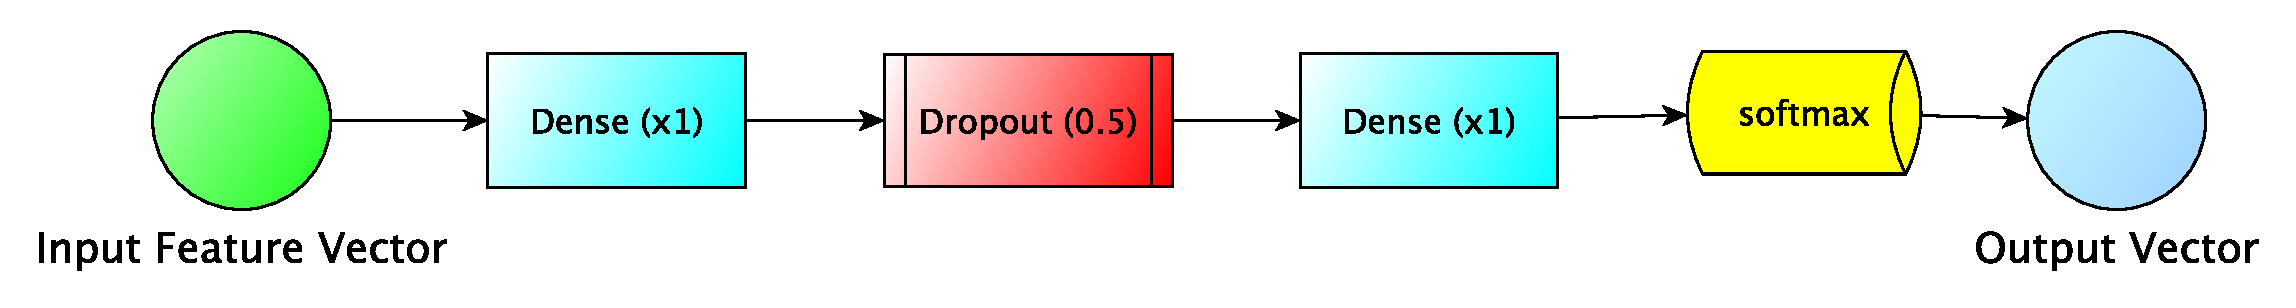
\includegraphics[width=0.85\textwidth]{figures/search_hh/mva/nn_arch_graph_updated}
        \caption{
            Illustration of the neural network graph employed in the analysis.
            The input feature vector has a length of 35 and the output vector is length 4,
            one for each of the targetted processes.
        }
        \label{fig:nn_arch}
    \end{center}
\end{figure}
Each of the dense layers are 250 nodes wide and  have their weights randomly initialized by sampling
from a truncated normal distribution centered on zero with a width given by $\sqrt{1/N_{\text{inputs}}}$, where
$N_{\text{inputs}}$ is the number of input features (the length of the input vector).
The activation functions for each of the dense layers are rectified linear units (`ReLu')~\cite{ReLu}.

Using an output layer with a softmax activation function allows one to interpret the outputs as
each representing a probability\footnote{The use of the term `probability' here is only
loosely correct, as the outputs are not \textit{strictly} probabilities.}
for the output's associated class ($hh$, Top, $Z \rightarrow \{ee,\mu\mu\}$,
or $Z \rightarrow \tau\tau$) given the inputs and for this reason it is commonly used for multi-class
neural network classifiers.
The association of the softmax activation with a class probability can be seen by its definition,
\begin{align}
    a_j = \frac{ e^{z_j} } { \sum\limits_k e ^{z_k} },
    \label{eq:softmax_activation}
\end{align}
where $a_j$ is the activation of the $j^{th}$ output neuron, the $z_i$ are the inputs to the output layer,
and $k$ runs over all output neurons.
It can be seen that if one sums over all outputs of a layer whose activation is given by Equation~\ref{eq:softmax_activation}
that the sum is equal to one.
Thus, the outputs of the softmax layer can be seen as a probability distribution.
For this reason, in the discussion to follow, we refer to the outputs of our neural network as `$p_i$',
where $i$ has four possibiities for each of the four outputs: $i \in \{ hh, \text{Top}, Z\rightarrow ee/\mu\mu, Z\rightarrow \tau\tau \}$.

The use of droput layers during the training process of is a form of statistical learning regularization that is reminiscient
of ensemble methods in the non-deep-learning arena, such as random forests~\cite{RandomForestsBreiman2001}.
They act to randomly disable a tunable fraction of inputs during various points in the training stage~\cite{JMLRDropout}.
This tunable fraction is referred to as the \textit{dropout rate}.
The use of dropout regularization prevents nodes within the network from co-adapting too much, thus reducing
the effects of overtraining.
This is illustrated in Figure~\ref{fig:dropout_illustration}.
During each batch of events forwarded to the network during the training phase, the dropout layer disables
portions of the network and thereby presents a modified network to the inputs.
Conceptually, then, using dropout during training is similar to training a set of very many, different \textit{weak}
neural networks.
During test time, at the time when the neural network is actually being used in the analysis,
the network's weights, which have been determined after training over the set of thinned networks,
are scaled down by the dropout rate.
This is illustrated in Figure~\ref{fig:dropout_weight_scaling}.

\begin{figure}[!htb]
    \begin{center}
        \includegraphics[width=0.85\textwidth]{figures/search_hh/mva/dropout_illustration}
        \caption{
            Illustration of dropout regularization. Figure taken from Ref.~\cite{JMLRDropout}.
            \textit{\textbf{Left}}: A standard neural network with two fully-connected layers.
            \textit{\textbf{Right}}: An example of a thinned network produced by applying dropout to the
                network on the left.
                The units with `X' have been dropped.
        }
        \label{fig:dropout_illustration}
    \end{center}
\end{figure}

\begin{figure}[!htb]
    \begin{center}
        \includegraphics[width=0.85\textwidth]{figures/search_hh/mva/dropout_weight_scaling}
        \caption{
            Illustration of the dropout rate effect on the network weights. Figure taken from Ref.~\cite{JMLRDropout}.
            \textit{\textbf{Left}}: A node in a fully-connected layer at training time is present in the network with
                a probability equal to the dropout rate and is connected to the next layer with weights represented by $\bm{w}$.
            \textit{\textbf{Right}}: At test time, the node is present with 100\% probability but its weights are scaled down by the
                dropout rate, $p\bm{w}$.
        }
        \label{fig:dropout_weight_scaling}
    \end{center}
\end{figure}

\noindent
As mentioned above, the use of dropout regularization prevents nodes within the network from co-adapting
too much and forces the network to learn more robust features that are useful in conjunction with many 
different random subsets of the other nodes.
That is, dropout regularization ensures that the model is robust against the loss of any individual
``piece of evidence'' and is found to reduce the effects of overtraining, which improves the generalizability
of the trained classifier.

The neural network classifier used in the present analysis, illustrated in Figure~\ref{fig:nn_arch},
uses a single dropout layer acting on the first fully-connected node and is given a dropout rate of 50\%.

During training, the loss metric is the categorical crossentropy and the Adam optimization algorithm~\cite{AdamOptimizer} is used.\footnote{More
on categorical cross-entropy: \href{https://ml-cheatsheet.readthedocs.io/en/latest/loss_functions.html\#cross-entropy}
{https://ml-cheatsheet.readthedocs.io/en/latest/loss\_functions.html\#cross-entropy}}


%%%%%%%%%%%%%%%%%%%%%%%%%%%%%%%%%%%%%%%%%%%%%%%%%%%%%%%%%%%%%%%%%%%%%%%%%%%%%%%%%%%
%%%%%%%%%%%%%%%%%%%%%%%%%%%%%%%%%%%%%%%%%%%%%%%%%%%%%%%%%%%%%%%%%%%%%%%%%%%%%%%%%%%
%%%%%%%%%%%%%%%%%%%%%%%%%%%%%%%%%%%%%%%%%%%%%%%%%%%%%%%%%%%%%%%%%%%%%%%%%%%%%%%%%%%
%
% TRAINING AND ARCHITECTURE
%
%%%%%%%%%%%%%%%%%%%%%%%%%%%%%%%%%%%%%%%%%%%%%%%%%%%%%%%%%%%%%%%%%%%%%%%%%%%%%%%%%%%
%%%%%%%%%%%%%%%%%%%%%%%%%%%%%%%%%%%%%%%%%%%%%%%%%%%%%%%%%%%%%%%%%%%%%%%%%%%%%%%%%%%
%%%%%%%%%%%%%%%%%%%%%%%%%%%%%%%%%%%%%%%%%%%%%%%%%%%%%%%%%%%%%%%%%%%%%%%%%%%%%%%%%%%

\section{Estimation of Backgrounds}
\label{sec:stop_background_estimate}

In this section, we describe the methods used for the estimation of the SM background
contamination in the SRs.
By Table~\ref{tab:stop_exp_sr_yield}, it can be seen that the expected SM background
contamination to the SRs in the \bWN search is primarily composed of events
from the \ttbar~and diboson processes.
Given that these are the dominant backgrounds for the analysis, their estimation is performed
using the control region method, described in Section~\ref{sec:control_region_method}.
That is, dedicated CRs and VRs are defined for each of the two processes in order
to provide a normalisation correction for their MC prediction in the SRs.
All other background processes, being subdominant, have their predicted contribution
to the SR background taken directly from the MC simulation.
The estimation of the contribution of sources leading to fake and non-prompt leptons
is performed using the Matrix Method, described in Section~\ref{sec:matrix_method}.

Sections~\ref{sec:stop_ttbar_estimate} and \ref{sec:stop_vv_estimate} describe
the background estimate for the \ttbar~and diboson processes, respectively.

%sub-dominant and FNP via MC alone (shape and normalisation prediction)
%dominant, ttbar and vv, are estimated in a semi-data driven fashion using
% dedicated control regions
%  --> yields tables in CR
%  --> SR normalisation correction factors

The CR and VR definitions for both the \ttbar~and diboson background are based on the
SR definitions given in the previous section.
The CRs are defined primarily by inverting the two-dimensional selection
made in the $(\cosb, \dpb)$-plane, and maintaining similar selections as in the SRs for the other variables.
The VRs, on the other hand, are defined by inverting the selections on the non-angular variables relative to those
made in the SRs.

\begin{figure}[!htb]
    \begin{center}
        \includegraphics[width=0.7\textwidth]{figures/search_stop2l/bkg_est/crvrmotivation}
        \caption{
            Illustration of the CR and VR strategy used in the \bWN search.
            The defining characteristic for the definition of these regions is
            based on the region in the $(\cosb, \dpb)$-plane that they select.
            The CR inverts the requirements on these quantities relative to the SRs,
            while the VR has the same requirements as in the SRs but inverts
            selections made on the other observables.
        }
        \label{fig:stop_crvr_motivation}
    \end{center}
\end{figure}

\FloatBarrier
%%%%%%%%%%%%%%%%%%%%%%%%%%%%%%%%%%%%%%%%%%%%%%%%%%%%%%%%%%%%%%%%%%%%%%%%%%%%%%%%%%%%%%%%%%%%
%%%%%%%%%%%%%%%%%%%%%%%%%%%%%%%%%%%%%%%%%%%%%%%%%%%%%%%%%%%%%%%%%%%%%%%%%%%%%%%%%%%%%%%%%%%%
%%%%%%%%%%%%%%%%%%%%%%%%%%%%%%%%%%%%%%%%%%%%%%%%%%%%%%%%%%%%%%%%%%%%%%%%%%%%%%%%%%%%%%%%%%%%
%
% TOP BKG
%
%%%%%%%%%%%%%%%%%%%%%%%%%%%%%%%%%%%%%%%%%%%%%%%%%%%%%%%%%%%%%%%%%%%%%%%%%%%%%%%%%%%%%%%%%%%%
%%%%%%%%%%%%%%%%%%%%%%%%%%%%%%%%%%%%%%%%%%%%%%%%%%%%%%%%%%%%%%%%%%%%%%%%%%%%%%%%%%%%%%%%%%%%
%%%%%%%%%%%%%%%%%%%%%%%%%%%%%%%%%%%%%%%%%%%%%%%%%%%%%%%%%%%%%%%%%%%%%%%%%%%%%%%%%%%%%%%%%%%%

\subsection{Top-quark pair production}
\label{sec:stop_ttbar_estimate}

The CRs and VRs designed to derive and validate the semi-data-driven
normalisation correction factor for the \ttbar~background process are called
CR-Top and VR-Top, respectively, and are defined in Table~\ref{tab:stop_top_crvr}.
The strategy for the CR and VR selections in the $(\cosb, \dpb)$ plane are described
in the previous section.
Several of the selections on the kinematic quantities relative to those in the SRs (c.f. Table~\ref{tab:stop_sr_def})
are relaxed.
In both CR-Top and VR-Top, the \mdr requirement is relaxed to $\mdr > 80$\,GeV and the requirement on the
\gaminv quantity is removed.
In VR-Top, the \rpt requirement is inverted relative to that used in the SRs.
Given that the \ttbar~background is flavor symmetric, only different-flavor events
are allowed to populate CR-Top and VR-Top, in order to avoid contamination from $Z$-boson processes.
As a result, no additioanl requirement on $m_{\ell\ell}$ is made in these regions.
For increased purity, CR-Top requires that there be at least one $b$-tagged jet,
while VR-Top applies a veto in order to be orthogonal to CR-Top.

VR-Top is defined to have zero $b$-tagged jets, while CR-Top requires at least one.
In dedicated studies, it has been verified that the \ttbar~normalisation correction derived
in the $b$-jet rich region CR-Top is well extrapolated to separate validation regions, and is rather
independent of the $b$-tagged jet multiplicity.
This gives confidence that VR-Top can be used as an appropriate check on the \ttbar~normalisation
correct factor and that it's extrapolation to the SRs, which have differing requirements on the
$b$-tagged jet multiplicity, is reasonable.

Distributions of several key observables in CR-Top are shown in Figures~\ref{fig:crt_0}-\ref{fig:crt_1}.
{\color{red}{VR-TOP DISTRIBUTIONS IN APPENDIX??}}

\begin{table}[!htb]
    \begin{center}
        \begin{scriptsize}
        \caption{
            Definitions of the CR and VR for the \ttbar~background process for the
            \bWN search.
        }
        \label{tab:stop_top_crvr}
        \begin{tabular}{l | c c}
            \hline
            \hline
                & \multicolumn{2}{c}{\textbf{Regions}} \\
            \hline
            \textbf{Variable} & \textbf{CR-Top} & \textbf{VR-Top} \\
            \hline
            Dilepton Flavor & DF & DF \\
            $m_{\ell\ell}$ [GeV]    & no req. & no req. \\
            Lead lepton \pT~[GeV] & $>25$ & $>25$ \\
            Sub-lead lepton \pT~[GeV] & $>20$ & $>20$ \\
            $b$-tagged jet multiplicity & $>0$ & Exactly 0 \\
            \mdr [GeV] & $>80$ & $>80$ \\
            \rpt & $>0.7$ & $<0.7$ \\
            \gaminv & no req. & no req. \\
            $(\cosb, \dpb)$ & \multicolumn{1}{c}{\small{$\dpb < 0.9 \times | \cosb | + 1.6$}} & \multicolumn{1}{c}{\small{$\dpb> 0.9 \times | \cosb | + 1.6$}} \\
            %$(\cosb, \dpb)$ & $\dpb $ & $\dpb$ \\
            %        & \hspace{1.8cm} $< 0.9 \times | \cosb | + 1.6$ & \hspace{1.8cm}$> 0.9 \times | \cosb | + 1.6$ \\
            \hline
            \hline
        \end{tabular}
        \end{scriptsize}
    \end{center}
\end{table}

\subsubsection{Kinematic Distributions in CR-Top}

\begin{figure}[!htb]
    \begin{center}
        \includegraphics[width=0.48\textwidth]{figures/search_stop2l/bkg_est/crtop/crt_MDR}
        \includegraphics[width=0.48\textwidth]{figures/search_stop2l/bkg_est/crtop/crt_l_pt0}
        \includegraphics[width=0.48\textwidth]{figures/search_stop2l/bkg_est/crtop/crt_DPB_vSS}
        \includegraphics[width=0.48\textwidth]{figures/search_stop2l/bkg_est/crtop/crt_cosThetaB}
        \caption{
            Distributions of \mdr (\textit{upper left}), leading lepton \pT~(\textit{upper right}),
            \dpb (\textit{lower left}), and $|\cosb|$ (\textit{lower right}) in the \ttbar CR,
            CR-Top.
            The error on the SM processes includes statistical and systematic uncertainties.
            The post-fit normalization correction factors for the \ttbar and diboson processes
            have been applied.
        }
        \label{fig:crt_0}
    \end{center}
\end{figure}
\begin{figure}[!htb]
    \begin{center}
        \includegraphics[width=0.48\textwidth]{figures/search_stop2l/bkg_est/crtop/crt_RPT}
        \includegraphics[width=0.48\textwidth]{figures/search_stop2l/bkg_est/crtop/crt_gamInvRp1}
        \includegraphics[width=0.48\textwidth]{figures/search_stop2l/bkg_est/crtop/crt_nBJets}
        \includegraphics[width=0.48\textwidth]{figures/search_stop2l/bkg_est/crtop/crt_nSJets}
        \caption{
            Distributions of \rpt (\textit{upper left}), leading lepton \gaminv~(\textit{upper right}),
            $b$-tagged jet multiplicity (\textit{lower left}), and non-$b$-tagged jet multiplicity(\textit{lower right}) in the \ttbar CR,
            CR-Top.
            The error on the SM processes includes statistical and systematic uncertainties.
            The post-fit normalization correction factors for the \ttbar and diboson processes
            have been applied.
        }
        \label{fig:crt_1}
    \end{center}
\end{figure}



%%%%%%%%%%%%%%%%%%%%%%%%%%%%%%%%%%%%%%%%%%%%%%%%%%%%%%%%%%%%%%%%%%%%%%%%%%%%%%%%%%%%%%%%%%%%
%%%%%%%%%%%%%%%%%%%%%%%%%%%%%%%%%%%%%%%%%%%%%%%%%%%%%%%%%%%%%%%%%%%%%%%%%%%%%%%%%%%%%%%%%%%%
%%%%%%%%%%%%%%%%%%%%%%%%%%%%%%%%%%%%%%%%%%%%%%%%%%%%%%%%%%%%%%%%%%%%%%%%%%%%%%%%%%%%%%%%%%%%
%
% VV BKG
%
%%%%%%%%%%%%%%%%%%%%%%%%%%%%%%%%%%%%%%%%%%%%%%%%%%%%%%%%%%%%%%%%%%%%%%%%%%%%%%%%%%%%%%%%%%%%
%%%%%%%%%%%%%%%%%%%%%%%%%%%%%%%%%%%%%%%%%%%%%%%%%%%%%%%%%%%%%%%%%%%%%%%%%%%%%%%%%%%%%%%%%%%%
%%%%%%%%%%%%%%%%%%%%%%%%%%%%%%%%%%%%%%%%%%%%%%%%%%%%%%%%%%%%%%%%%%%%%%%%%%%%%%%%%%%%%%%%%%%%

\subsection{Diboson Production}
\label{sec:stop_vv_estimate}

The SM diboson processes are composed of $WW$, $ZW+WZ$, and $ZZ$ production.
The dominant process for the \bWN SRs is $WW$, as discussed in the text.
In order to constrain the $WW$ component, in addition to those components with a $Z$ boson,
the diboson CRs are split into two, one targetting the different-flavor enriched component
of the diboson background (predominantly $WW$) and one in which the same-flavor component ($ZW+WZ$ and $ZZ$)
is enriched.

The same-flavor and different-flavor diboson CRs (VRs), CR-VV-SF and CR-VV-DF (VR-VV-SF and VR-VV-DF), respectively,
are defined in Table~\ref{tab:stop_vv_crvr}.
All of the regions apply a $b$-tagged jet veto.
Although there are SRs that are inclusive of $b$-tagged jets (SRt-SF and SRt-DF), the diboson background
is negligible in them and so the normalisation correction factors derived in the diboson CRs
can be extrapolated with confidence into the SRs with a $b$-tagged jet veto (SRw-SF and SRw-DF).
There is no difference between the same-flavor and different-flavor CRs, apart from the dilepton flavor
requirements and $Z$-veto.
The diboson VRs have the same, or inclusive, \rpt and \gaminv  selections as the CRs but have orthogonal
\mdr requirements that move them closer the SR selections.

Distributions of several key observables in CR-VV-SF (CR-VV-DF) are shown in Figures~\ref{fig:crvvSF_0}-\ref{fig:crvvSF_1}
(Figures~\ref{fig:crvvDF_0}-\ref{fig:crvvDF_1}).

{\color{red}{VR-VV DISTRIBUTIONS IN APPENDIX??}}

\begin{table}[!htb]
    \begin{center}
        \begin{scriptsize}
        \caption{
            Definitions of the CR and VR for the diboson~background processes for the
            \bWN search.
        }
        \label{tab:stop_vv_crvr}
        \begin{tabular}{l | c c c c}
            \hline
            \hline
                & \multicolumn{4}{c}{\textbf{Regions}} \\
            \hline
            \textbf{Variable} & \textbf{CR-VV-DF} & \textbf{CR-VV-SF} & \textbf{VR-VV-DF} & \textbf{VR-VV-SF} \\
            \hline
            Dilepton Flavor & DF & SF & DF & SF \\
            $m_{\ell\ell}$ [GeV]    & no req. & $|m_{\ell\ell} - 91.2| > 10$ & no req. & $|m_{\ell\ell} - 91.2| > 10$ \\
            Lead lepton \pT~[GeV] & $>25$ & $>25$ & $>25$ & $>25$ \\
            Sub-lead lepton \pT~[GeV] & $>20$ & $>20$ & $>20$ & $>20$ \\
            $b$-tagged jet multiplicity & Exactly 0 & Exactly 0 & Exactly 0 & Exactly 0 \\
            \mdr [GeV] & $>50$ & $>70$ & $\in(50,95)$ & $\in(60,95)$ \\
            \rpt & $<0.5$ & $<0.5$ & $<0.7$ & $<0.4$ \\
            \gaminv &  $>0.7$ & $>0.7$ & $>0.7$ & $>0.7$ \\
            $(\cosb, \dpb)$ & \multicolumn{2}{c}{\small{$\dpb < 0.9 \times | \cosb | + 1.6$}} & \multicolumn{2}{c}{\small{$\dpb> 0.9 \times | \cosb | + 1.6$}} \\
%            $(\cosb, \dpb)$ & $\dpb $  &  $\dpb$ & \\
%                    & \hspace{1.8cm} $< 0.9 \times | \cosb | + 1.6$  & \hspace{1.8cm}$> 0.9 \times | \cosb | + 1.6$ \\
            \hline
            \hline
        \end{tabular}
        \end{scriptsize}
    \end{center}
\end{table}

\begin{figure}[!htb]
    \begin{center}
        \includegraphics[width=0.48\textwidth]{figures/search_stop2l/bkg_est/crvsf/crvSF_MDR}
        \includegraphics[width=0.48\textwidth]{figures/search_stop2l/bkg_est/crvsf/crvSF_l_pt0}
        \includegraphics[width=0.48\textwidth]{figures/search_stop2l/bkg_est/crvsf/crvSF_DPB_vSS}
        \includegraphics[width=0.48\textwidth]{figures/search_stop2l/bkg_est/crvsf/crvSF_cosThetaB}
        \caption{
            Distributions of \mdr (\textit{upper left}), leading lepton \pT~(\textit{upper right}),
            \dpb (\textit{lower left}), and $|\cosb|$ (\textit{lower right}) in the same-flavor diboson CR,
            CR-VV-SF.
            The error on the SM processes includes statistical and systematic uncertainties.
            The post-fit normalization correction factors for the \ttbar and diboson processes
            have been applied.
        }
        \label{fig:crvvSF_0}
    \end{center}
\end{figure}
\begin{figure}[!htb]
    \begin{center}
        \includegraphics[width=0.48\textwidth]{figures/search_stop2l/bkg_est/crvsf/crvSF_RPT}
        \includegraphics[width=0.48\textwidth]{figures/search_stop2l/bkg_est/crvsf/crvSF_gamInvRp1}
        \includegraphics[width=0.48\textwidth]{figures/search_stop2l/bkg_est/crvsf/crvSF_nBJets}
        \includegraphics[width=0.48\textwidth]{figures/search_stop2l/bkg_est/crvsf/crvSF_nSJets}
        \caption{
            Distributions of \rpt (\textit{upper left}), leading lepton \gaminv~(\textit{upper right}),
            $b$-tagged jet multiplicity (\textit{lower left}), and non-$b$-tagged jet multiplicity(\textit{lower right}) in the same-flavor diboson CR,
            CR-VV-SF.
            The error on the SM processes includes statistical and systematic uncertainties.
            The post-fit normalization correction factors for the \ttbar and diboson processes
            have been applied.
        }
        \label{fig:crvvSF_1}
    \end{center}
\end{figure}

\begin{figure}[!htb]
    \begin{center}
        \includegraphics[width=0.48\textwidth]{figures/search_stop2l/bkg_est/crvdf/crv_MDR}
        \includegraphics[width=0.48\textwidth]{figures/search_stop2l/bkg_est/crvdf/crv_l_pt0}
        \includegraphics[width=0.48\textwidth]{figures/search_stop2l/bkg_est/crvdf/crv_DPB_vSS}
        \includegraphics[width=0.48\textwidth]{figures/search_stop2l/bkg_est/crvdf/crv_cosThetaB}
        \caption{
            Distributions of \mdr (\textit{upper left}), leading lepton \pT~(\textit{upper right}),
            \dpb (\textit{lower left}), and $|\cosb|$ (\textit{lower right}) in the different-flavor diboson CR,
            CR-VV-DF.
            The error on the SM processes includes statistical and systematic uncertainties.
            The post-fit normalization correction factors for the \ttbar and diboson processes
            have been applied.
        }
        \label{fig:crvvDF_0}
    \end{center}
\end{figure}
\begin{figure}[!htb]
    \begin{center}
        \includegraphics[width=0.48\textwidth]{figures/search_stop2l/bkg_est/crvdf/crv_RPT}
        \includegraphics[width=0.48\textwidth]{figures/search_stop2l/bkg_est/crvdf/crv_gamInvRp1}
        \includegraphics[width=0.48\textwidth]{figures/search_stop2l/bkg_est/crvdf/crv_nBJets}
        \includegraphics[width=0.48\textwidth]{figures/search_stop2l/bkg_est/crvdf/crv_nSJets}
        \caption{
            Distributions of \rpt (\textit{upper left}), leading lepton \gaminv~(\textit{upper right}),
            $b$-tagged jet multiplicity (\textit{lower left}), and non-$b$-tagged jet multiplicity(\textit{lower right}) in the different-flavor diboson CR,
            CR-VV-DF.
            The error on the SM processes includes statistical and systematic uncertainties.
            The post-fit normalization correction factors for the \ttbar and diboson processes
            have been applied.
        }
        \label{fig:crvvDF_1}
    \end{center}
\end{figure}

\FloatBarrier
%%%%%%%%%%%%%%%%%%%%%%%%%%%%%%%%%%%%%%%%%%%%%%%%%%%%%%%%%%%%%%%%%%%%%%%%%%%%%%%%%%%%%%%%%%%%
%%%%%%%%%%%%%%%%%%%%%%%%%%%%%%%%%%%%%%%%%%%%%%%%%%%%%%%%%%%%%%%%%%%%%%%%%%%%%%%%%%%%%%%%%%%%
%%%%%%%%%%%%%%%%%%%%%%%%%%%%%%%%%%%%%%%%%%%%%%%%%%%%%%%%%%%%%%%%%%%%%%%%%%%%%%%%%%%%%%%%%%%%
%
% POST FIT
%
%%%%%%%%%%%%%%%%%%%%%%%%%%%%%%%%%%%%%%%%%%%%%%%%%%%%%%%%%%%%%%%%%%%%%%%%%%%%%%%%%%%%%%%%%%%%
%%%%%%%%%%%%%%%%%%%%%%%%%%%%%%%%%%%%%%%%%%%%%%%%%%%%%%%%%%%%%%%%%%%%%%%%%%%%%%%%%%%%%%%%%%%%
%%%%%%%%%%%%%%%%%%%%%%%%%%%%%%%%%%%%%%%%%%%%%%%%%%%%%%%%%%%%%%%%%%%%%%%%%%%%%%%%%%%%%%%%%%%%

\subsection{Background-only Fit}
\label{sec:stop_background_only}

In order to assess the impact of the CRs on the background estimation in the SRs, a so-called `background-only'
fit is performed.
A background-only fit is profile-likelihood fit, as described Section~\ref{sec:likelihood},
in which the only regions contributing to the likelihood (c.f Equation~\ref{eq:full_likelihood})
are the analysis' CRs.
The result of running a background-only fit to data in the CRs is shown in Table~\ref{tab:bkgonly_CRVR},
which shows the MC predicted yields for the background processes both before and after the
background-only fit is performed, as well as the observed data counts, in each of the CRs and VRs in the analysis.
The post-fit yields in the CRs are expected to agree with the observed data counts, since the latter are used
as constraints in the fit model and there are as many freely-floating parameters in the fit (3 $\mu$ factors)
as there are CRs; therefore, the fit has enough freedom to cover any discrepancy between the observed data and pre-fit MC prediction of
the background processes.
The agreement observed between the post-fit MC and the observed data in the VRs shows that the extrapolation,
at least in terms of the corrected MC's normalisation, is performing well.

The normalisation correction factors for the \ttbar~and diboson processes obtained in the background-only
fit are listed in Table~\ref{tab:stop_scalefactors}.
They are generally consistent with one.

\begin{table}[!htb]
\begin{center}
\setlength{\tabcolsep}{0.0pc}
{\scriptsize
\caption{
Yields in the \ttbar~and diboson CRs and VRs for the \bWN search for the main background processes
contributing to the analysis.
The lower-portion of the table are the yields before the background-only fit to data
in the CRs, without the normalisation corrections applied.
The upper-portion of the table are those taken after the background-only fit to data.
The errors on the quoted numbers are due to the statistical and experimental systematic uncertainties.
}
\label{tab:bkgonly_CRVR}
\begin{tabular*}{\textwidth}{@{\extracolsep{\fill}}lrrrrrr}
\noalign{\smallskip}\hline\noalign{\smallskip}
\noalign{\smallskip}\hline\noalign{\smallskip}
\textbf{Process}           & \textbf{CR-Top}            & \textbf{CR-VV-DF}            & \textbf{CR-VV-SF}            & \textbf{VR-Top}           & \textbf{VR-VV-DF}            & \textbf{VR-VV-SF}              \\[-0.05cm]
\noalign{\smallskip}\hline\noalign{\smallskip}


Observed Data         & $951$              & $2046$              & $1275$              & $1197$              & $1896$              & $783$                    \\
\noalign{\smallskip}\hline\noalign{\smallskip}
%%
Post-fit Total SM         & $951.00 \pm 30.84$          & $2046.05 \pm 45.23$          & $1275.17 \pm 35.68$          & $1231.78 \pm 86.59$          & $2013.57 \pm 116.49$          & $780.44 \pm 117.32$              \\
\noalign{\smallskip}\hline\noalign{\smallskip}
%%
        Post-fit \ttbar          & $833.03 \pm 32.85$          & $619.74 \pm 111.40$          & $333.62 \pm 60.91$          & $733.87 \pm 64.91$          & $754.94 \pm 78.17$          & $127.14 \pm 22.09$              \\
%%
        Post-fit Diboson (DF)          & $11.51 \pm 2.43$          & $1093.28 \pm 125.83$          & $0.00 \pm 0.00$          & $331.13 \pm 82.57$          & $886.53 \pm 168.16$          & $0.00 \pm 0.00$              \\
%%
        Post-fit Diboson (SF)          & $0.00 \pm 0.00$          & $0.00 \pm 0.00$          & $378.94 \pm 124.32$          & $0.00 \pm 0.00$          & $0.00 \pm 0.00$          & $380.00 \pm 141.58$              \\
%%
        Post-fit Single-top          & $101.10 \pm 9.73$          & $186.47 \pm 27.99$          & $103.47 \pm 17.43$          & $111.52 \pm 14.49$          & $151.88 \pm 14.37$          & $36.40 \pm 5.62$              \\
%%
        Post-fit $\ttbar+V$          & $4.35 \pm 0.42$          & $0.39 \pm 0.07$          & $0.36 \pm 0.07$          & $1.27 \pm 0.22$          & $0.42 \pm 0.13$          & $0.05 \pm 0.02$              \\
%%
        Post-fit $Z$+jets          & $0.70 \pm 0.22$          & $1.83_{-1.83}^{+2.55}$          & $428.58 \pm 92.55$          & $0.47_{-0.47}^{+0.85}$          & $0.39_{-0.39}^{+0.71}$          & $191.37 \pm 78.38$              \\
%%
        Post-fit Single-higgs          & $0.31 \pm 0.13$          & $78.95 \pm 9.17$          & $6.23 \pm 1.06$          & $0.44_{-0.44}^{+0.52}$          & $54.98 \pm 4.34$          & $9.40 \pm 1.11$              \\
%%
        Post-fit Fakes          & $0.00 \pm 0.00$          & $65.37 \pm 2.22$          & $23.96 \pm 1.25$          & $53.09 \pm 1.92$          & $164.42 \pm 5.68$          & $36.09 \pm 3.04$              \\
%%
 \noalign{\smallskip}\hline\noalign{\smallskip}
%%
 Total SM               & $905.14 \pm 16.54$          & $1988.38 \pm 110.43$          & $1248.21 \pm 123.42$          & $1184.39 \pm 71.23$          & $1952.92 \pm 61.72$          & $764.65 \pm 99.06$              \\
\noalign{\smallskip}\hline\noalign{\smallskip}
%%
         \ttbar          & $787.43 \pm 11.29$          & $585.87 \pm 102.00$          & $315.39 \pm 55.87$          & $693.71 \pm 53.51$          & $713.64 \pm 66.57$          & $120.19 \pm 20.17$              \\
%%
         Diboson (DF)          & $11.25 \pm 1.62$          & $1069.46 \pm 12.45$          & $0.00 \pm 0.00$          & $323.89 \pm 50.27$          & $867.18 \pm 77.75$          & $0.00 \pm 0.00$              \\
%%
         Diboson (SF)          & $0.00 \pm 0.00$          & $0.00 \pm 0.00$          & $370.13 \pm 15.48$          & $0.00 \pm 0.00$          & $0.00 \pm 0.00$          & $371.16 \pm 34.38$              \\
%%
         Single-top          & $101.10 \pm 9.80$          & $186.49 \pm 28.25$          & $103.49 \pm 17.59$          & $111.52 \pm 14.60$          & $151.88 \pm 14.46$          & $36.41 \pm 5.66$              \\
%%
         $\ttbar+V$          & $4.35 \pm 0.42$          & $0.39 \pm 0.07$          & $0.36 \pm 0.07$          & $1.27 \pm 0.23$          & $0.42 \pm 0.13$          & $0.05 \pm 0.02$              \\
%%
         $Z$+jets          & $0.70 \pm 0.23$          & $1.83_{-1.83}^{+2.57}$          & $428.65 \pm 93.15$          & $0.48_{-0.48}^{+0.86}$          & $0.40_{-0.40}^{+0.72}$          & $191.36 \pm 78.78$              \\
%%
         Single-higgs          & $0.31 \pm 0.13$          & $78.96 \pm 9.26$          & $6.23 \pm 1.07$          & $0.44_{-0.44}^{+0.53}$          & $54.98 \pm 4.37$          & $9.40 \pm 1.12$              \\
%%
         Fakes          & $0.00 \pm 0.00$          & $65.37 \pm 2.23$          & $23.96 \pm 1.26$          & $53.09 \pm 1.92$          & $164.42 \pm 5.70$          & $36.09 \pm 3.04$              \\
\noalign{\smallskip}\hline\noalign{\smallskip}
\noalign{\smallskip}\hline\noalign{\smallskip}
\end{tabular*}
}
\end{center}
\end{table}

\begin{table}[!htb]
    \begin{center}
        \caption{
            Normalisation correction factors for the \ttbar~$(\mu_{\ttbar})$,
            same-flavor diboson $(\mu_{\text{VV-SF}})$, and different-flavor diboson $(\mu_{\text{VV-DF}})$
            processes derived from the background-only fit to the CRs.
            The errors on the quoted numbers are due to the statistical and experimental systematic uncertainties
            entering the fit.
        }
        \label{tab:stop_scalefactors}
        \begin{tabular}{l|c}
            \hline
            \hline
                $\mu_{\ttbar}$ & $1.06 \pm 0.05$ \\
                $\mu_{\text{VV-SF}}$ & $1.02 \pm 0.12$ \\
                $\mu_{\text{VV-DF}}$ & $1.02 \pm 0.35$ \\
            \hline
            \hline
        \end{tabular}
    \end{center}
\end{table}


\section{Results}
\label{sec:stop_results}


%\chapter{Concluding Remarks}
\label{chap:conclusion}

%\epigraph{
%\textit{When information is cheap, attention becomes expensive.}
%}
%{
%--James Gleick, \textit{The Information}
%}
%
%\epigraph{
%\textit{Our task as men is to find the few principles that will calm the infinite anguish
%of free souls. We must mend what has been torn apart, make justice imaginable again in a
%world so obviously unjust, give happiness a meaning once more to peoples poisoned by the
%misery of the century. Naturally, it is a superhuman task. But superhuman is the term
%for tasks men take a long time to accomplish, that's all.}
%}
%{
%--Albert Camus, \textit{The Almond Trees}
%}

\epigraph{
    \textit{The point is there ain't no point.}
}
{
    --Cormac McCarthy, \textit{No Country for Old Men}
}

%\epigraph{
%    \textit{The more the universe seems comprehensible, the more it also seems pointless.
%    But if there is no solace in the fruits of our research, there is at least some consolation
%    in the research itself. Men and women are not content to comfort themselves with tales of
%    gods and giants, or to confine their thoughts to the daily affairs of life; they also build telescopes
%    and satellites and accelerators, and sit at their desks for endless hours working out the meaning of the
%    data they gather. The effort to understand the universe is one of the very few things that lifts
%    human life a little above the level of farce, and gives it some of the grace of tragedy.}
%}
%{
%    --Steven Weinberg, \textit{The First Three Minutes}
%}

\epigraph{
    \textit{The effort to understand the universe is one of the very few things that lifts
    human life a little above the level of farce, and gives it some of the grace of tragedy.}
}
{
    --Steven Weinberg, \textit{The First Three Minutes}
}

%%%%%%%%%%%%%%%%%%%%%%%%%%%%%%%%%%%%%%%%%%%%%%%%%%%%%%%%%%%%%%%%%%%%%%%%%%%%%%%%%%%%%%%%%%%%%%
%%%%%%%%%%%%%%%%%%%%%%%%%%%%%%%%%%%%%%%%%%%%%%%%%%%%%%%%%%%%%%%%%%%%%%%%%%%%%%%%%%%%%%%%%%%%%%
%%%%%%%%%%%%%%%%%%%%%%%%%%%%%%%%%%%%%%%%%%%%%%%%%%%%%%%%%%%%%%%%%%%%%%%%%%%%%%%%%%%%%%%%%%%%%%

\cite{FengNaturalness}

This dissertation has presented work related to the on-going upgrade of the forward muon system
of the ATLAS detector --- the New Small Wheel --- as well as two searches for BSM physics in dilepton final states.
The work thus described has taken place within the years 2015--2019, containing the entirety of the LHC Run 2,
and during a time of change in the physics program of the ATLAS experiment.

At the time of writing in October 2019, the NSW project is on a critical path, at least with respect to its initial timeline of
being fully constructed and installed in ATLAS within the Phase 1 upgrade (c.f. Figure~\ref{fig:lh_schedule}).
In the past few years, the NSW project has seen significant delays.
The construction of large-scale MM and sTGC detectors has never been done prior to the NSW, and
understanding the construction process and behavior of these detectors has been a challenging process
that has, at times, required halting chamber production in order to understand emergent phenomena
that had not been foreseen.
The entire suite of frontend electronics has seen issues, as well, with one of the predominant issues being related to the
design of the ASICs themselves.
The important readout ASIC, the VMM, has had to go through at least one unforeseen design fix to address
issues discovered in the lab, for example.
Even at the time of writing, the current understanding of the yield\footnote{The term `yield' here means
the fraction of produced VMMs that meet the performance criteria for being sufficient for use in ATLAS, and are not
failing specific criteria that are necessary in order to meet the physics goals of ATLAS.}
of the latest version of the VMM ASIC production is unknown.
Understanding this is currently of the utmost priority, since the frontend board development and construction of
detector chambers rely first on their being VMMs on-hand before they themselves can move forward and be fully commissioned.
If this yield is too low, additional ASICs will have to be manufactured at the silicon foundries, which is a lengthy process.
Additionally, the NSW will be the first subsystem of ATLAS to use the upgraded TDAQ system based
on the Front-end Link Exchange (FELIX)~\cite{FELIX} backend.
FELIX, itself, has seen significant delays in its Phase 1 upgrade progress that have led to 
further slowing the progress of the NSW.
With this in mind, the current best foreseen Phase 1 installation plan for the NSW project will be to install only a single wheel
into ATLAS before the start of LHC Run 3, with the second wheel being installed at some point
during Run 3, perhaps during one of the winter shutdown periods.
It may be likely that neither wheels is installed during Phase 1, at which point both wheels will have to be scheduled
for installation in Run 3.
The NSW is a very ambitious project, and such issues as described here are not indicative of those
at the heart of moving it forward but rather a sign of the short window of time that the project
was aiming to be completed in, as well as its having started at a time of great busyness and distraction
at CERN.
% given that the start of the LHC and Higgs discovery happened so near the early days of the NSW project's start.
%had as its goal as well as its having started at a time of great busyness and distraction at CERN, what with the start
%of the LHC and Higgs discovery happening at the time that the NSW as a project was starting.
The current author looks forward to its complete commissioning and smooth operation within the ATLAS experimental cavern,
which will be a testament to the hard work of many, many talented people from around the world having worked together
and designed, built, and butted-heads against a massive project of both new ideas and technologies.


\begin{figure}[!htb]
    \begin{center}
        \includegraphics[width=0.85\textwidth]{figures/conclusion/ATLAS_SUSY_Stop_tLSP}
        \caption{
        }
        \label{fig:run2_stop_summary}
    \end{center}
\end{figure}


%\chapter{The Standard Model of Particle Physics}

%\epigraph{\textit{So it goes...}}{---Kurt Vonnegut, \textit{Slaughterhouse
%		Five}}
	
%\epigraph{\textit{Science is a miracle.}}{--Ron Swanson}

\epigraph{\textit{If you wish to make an apple pie from scratch, you must first invent the universe.}}{--Carl Sagan, \textit{Cosmos: A Personal Voyage}}


As it stands, what has become known as the `Standard Model (SM) of Particle Physics'
is nothing less than one of the greatest achievments of mankind, due to both
the magnitude by which it has changed our perception of the underlying
nature of the universe and to the clever methods and tinkerings by which this
nature was unveiled by many clever physicists whose history has become veritable lore.
In terms of imagination and insight, it is second only to the special and general theories of relativity --
though the fields are nevertheless intricately intertwined.
%{\color{red}{The latter, though, being put forth by essentially a single person and the latter by a great many...}}.

Not considering the scientific progress made in the $18^{th}$ and $19^{th}$ centuries, and
ignoring the ancient Greeks despite their fabled invention of atomic theory,
the physical insights and major work that led to the current picture of elementary particle
physics described by the SM began with the \textit{annus mirabilis} papers of Albert
Einstein in the year 1905~\cite{einsteinPEE,einsteinSpecial,einsteinEnergyMass}.
In these papers, Einstein was able to shed light on the quantization of electromagnetic
radiation (building off of the seminal work of Max Planck~\cite{planckBlackBody})
and introduce the special theory of relativity.
These works laid the conceptual
and philosophical groundwork for the major breakthroughs in fundamental physics
of $20^{th}$ century physics: from the `old quantum theory' of Bohr and Sommerfeld
in the early 1900's to the equivalent wavefunction and matrix-mechanics formulations
of Schr{\"o}dinger and Heisenberg that
coalesced into `modern' quantum mechanics in the mid 1920's.
The modern approach, non-relativistic at its heart, provided a sufficient mathematical
and interpretable framework in which to work and match predictions to observed phenomena, old
and new. It has for the most part remained unchanged and is the quantum mechanics that is taught to
students at both the undergraduate and graduate level to this very day.
It is the theory that has since revolutionised all aspects of the physical sciences and
technologies that dictate our everyday-lives.
In the mid-1920's, however, despite
large efforts put forth by the forbears of modern quantum mechanics, the quantum-mechanical
world had yet to be made consistent with Einstein's theory of relativity --- a requirement
that must be met for all consistent physical theories of nature.
It was the insight of Paul Dirac who was finally able to successfully
marry the theory of the quantum with that of relativity when he introduced
his relativistic quantum-mechanical treatment of the electron in 1927 and 1928~\cite{diracEquation,Dirac:1927dy}.\footnote{
A complete history of the people and ideas involved in the development of the modern
theory of Quantum Mechanics can be found in references ~\cite{boffiRiseOfQM,historyQM},
and the references therein.
}
This work provided the starting point for a decades-long search of a consistent quantum-mechanical
and relativistic treatment of electrodynamics, known as \textit{quantum electrodynamics} (QED).
The search for QED ended at the end of the 1940's with the groundbreaking work of Dyson, Feynman, Schwinger, and Tomanaga~\cite{qedTomonaga,qedFeynman0,qedFeynman1,qedFeynman2,qedSchwinger0,qedSchwinger1,qedDyson0,qedDyson1} that introduced the covariant and gauge invariant
formulation of QED --- the first such relativistic quantum field theory (QFT).
QED allowed the phsycists to make predictions that agreed with observation to unprecedented levels
of accuracy and has since led to the adoption of its language and mathematical toolkit as the
foundational framework in which to construct models that accurately describe nature.\footnote{
	For a complete discussion of the developments leading up to QED, see the fabulous
	book by S. Schweber~\cite{Schweber:1994qa}.	
}
The SM is no less than an ultimate conclusion of these works: a consistent set of relativistic
quantum field theories, using the language developed by Feynman et al.,
that describes essentially all aspects of the known particles and forces that make up the 
observed universe.


\section{Particles and Forces}

Here we introduce the SM particle content and provide a description of the interactions that
link the particles together.


\begin{table}[!htb]
    \caption{
        The particle content of the SM and their transformation
        properties under the SM gauge groups, prior to electroweak symmetry breaking.
        The representations of each of the gauge groups are shown in the three-right
        columns. The \Uone symmetry of weak-hypercharge transformations is one-dimensional
        and the column gives the weak-hypercharge $\mathcal{Y}$ associated with each
        field. For \SUthree and \SUtwo, $\mathbf{1}$ refers to the field belonging to
        the associated singlet representation, $\mathbf{2}$ to the doublet representation,
        $\mathbf{3}$ to the triplet representation, and $\mathbf{8}$ to the octet representation.
    }
    \begin{center}
        \begin{tabularx}{0.96\textwidth}{m{1em} c c c c c c }
        \toprule
        \hline
        & Field Label & Content & Spin & \Uone~($\mathcal{=Y}$) & \SUtwo & \SUthree \\
        \hline
        \rotatebox{90}{\hspace{-0.1cm}\textbf{Quarks} } 
         &   \makecell{\fieldQi \\ \fieldUri \\ \fieldDri} % FIELD
         &   \makecell{ (\fieldUl, \fieldDl), (\fieldCl, \fieldSl), (\fieldTl, \fieldBl) \\ \fieldUr \\ \fieldDr}% CONTENT
         &   \makecell{ $1/2$ \\ $1/2$ \\ $1/2$} % SPIN
         &   \makecell{ $1/6$ \\ $2/3$ \\ $-1/3$}% U(1)
         &   \makecell{ $\mathbf{2}$ \\ $\mathbf{1}$ \\ $\mathbf{1}$}% SU(2)
         &   \makecell{ $\mathbf{3}$ \\ $\mathbf{3}$ \\ $\mathbf{3}$}\\ % SU(3)
        %\cdashline{1-7}
        \rotatebox{90}{\hspace{-0.1cm}\textbf{Leptons} }
         &   \makecell{\fieldLi \\ \fieldEri} % FIELD
         &   \makecell{ (\fieldEl, \fieldNuEl), (\fieldMul, \fieldNuMul), (\fieldTaul, \fieldNuTaul) \\ \fieldEr, \fieldMur, \fieldTaur}% CONTENT
         &   \makecell{ $1/2$ \\ $1/2$ }% SPIN
         &   \makecell{ $1/2$ \\ $-1$ }% U(1)
         &   \makecell{ $\mathbf{2}$ \\ $\mathbf{1}$ }% SU(2)
         &   \makecell{ $\mathbf{1}$ \\ $\mathbf{1}$ } \\ % SU(3)
        \midrule
        \rotatebox{90}{\textbf{\stackanchor{Gauge}{Fields}} }
         &   \makecell{\fieldB \\ \fieldW \\ \fieldG } % FIELD
         &   \makecell{ \fieldB \\ (\fieldWone, \fieldWtwo, \fieldWthree) \\ \fieldG$_a$, $a\in[1,..,8]$ }% CONTENT
         &   \makecell{ $1$ \\ $1$ \\ $1$} % SPIN
         &   \makecell{ $0$ \\ $0$ \\ $0$}% U(1)
         &   \makecell{ $\mathbf{1}$ \\ $\mathbf{3}$ \\ $\mathbf{1}$}% SU(2)
         &   \makecell{ $\mathbf{1}$ \\ $\mathbf{1}$ \\ $\mathbf{8}$}\\ % SU(3)
        \midrule
        \rotatebox{90}{\textbf{\stackanchor{Higgs}{Field}}} 
         &   \makecell{\fieldPhi } % FIELD
         &   \makecell{ (\fieldPhip, \fieldPhizero) }% CONTENT
         &   \makecell{ $0$  } % SPIN
         &   \makecell{ $1/2$  }% U(1)
         &   \makecell{ $\mathbf{2}$ }% SU(2)
         &   \makecell{ $\mathbf{1}$ }\\ % SU(3)
        \hline
        \bottomrule
        \end{tabularx}
    \end{center}
    \label{tab:sm_content}
\end{table}
\floatbarrier


\begin{table}[!htb]
    \caption{
        The particle content of the SM after the process of
        electroweak symmetry breaking.
    }
    \begin{center}
        \begin{tabularx}{1\textwidth}{m{1em} c c c c }
        \toprule
        \hline
        & Physical Field & Q & Coupling & Mass [GeV] \\
        \hline
        \rotatebox{90}{\hspace{-0.1cm}\textbf{Quarks} } 
            & \makecell{ \quarkU, \quarkC, \quarkT \\ \quarkD, \quarkS, \quarkB} % FIELD
            & \makecell{ $2/3$ \\ $-1/3$ }% Q
            %& \makecell{ $\mathbf{3}$ \\ $\mathbf{3}$ } % SU(3)
            & \makecell{ ($y_i=$) $1\times10^{-5}$, $7\times10^{-3}$, $1$ \\ ($y_i=$) $3\times10^{-5}$, $5\times10^{-4}$, $0.02$ } % Coupling
            & \makecell{ $2\times10^{-3}$, $1.27$, $173$ \\ $4\times10^{-4}$, $0.10$, $4.18$ }\\% Mass
        \rotatebox{90}{\hspace{-0.1cm}\textbf{Leptons} } 
            & \makecell{ \leptonE, \leptonMu, \leptonTau \\ \neutrinoE, \neutrinoMu, \neutrinoTau } % FIELD
            & \makecell{ $-1$ \\ $0$ }% Q
            %& \makecell{ $\mathbf{1}$ \\ $\mathbf{1}$ } % SU(3)
            & \makecell{ ($y_i=$) $3\times10^{-7}$, $6\times10^{-4}$, $0.01$ \\ -- } % Coupling
            & \makecell{ $5\times10^{-4}$, $0.106$, $1.777$ \\ --}\\% Mass
        \midrule
        \rotatebox{90}{\textbf{Bosons} } 
            & \makecell{ \fieldPhoton \\ \fieldZ \\ (\fieldWp, \fieldWm) \\ \fieldG } % FIELD
            & \makecell{ $0$ \\ $0$ \\ $(+1,-1)$ \\ $0$ }% Q
            %& \makecell{ $\mathbf{1}$ \\ $\mathbf{1}$ \\ $\mathbf{1}$ \\ $\mathbf{8}$ } % SU(3)
            & \makecell{ $\alpha_{\text{EM}} \simeq 1/137$ \\ $\sin \theta_{W} \simeq 0.5$ \\ -- \\ $\alpha_s \simeq 0.1$ } % Coupling
            & \makecell{ $0$ \\ $91.2$ \\ $80.4$ \\  $0$}\\% Mass
        \midrule
        \rotatebox{90}{\textbf{Higgs} } 
            & \makecell{ \fieldH } % FIELD
            & \makecell{ $0$ }% Q
            %& \makecell{ $\mathbf{1}$ } % SU(3)
            & \makecell{ $\lambda$, $\mu$ } % Coupling
            & \makecell{ $125.09$ }\\% Mass
        \hline
        \bottomrule
        \end{tabularx}
    \end{center}
    \label{tab:sm_content}
\end{table}



\subsection{Gauge Theories}

\subsubsection{The Electroweak Theory}



%\chapter{Experimental Setup}

%\epigraph{\textit{So it goes...}}{---Kurt Vonnegut, \textit{Slaughterhouse
%		Five}}
	
%\epigraph{\textit{Science is a miracle.}}{--Ron Swanson}

%\epigraph{\textit{If you wish to make an apple pie from scratch, you must first invent the universe.}}{--Carl Sagan, \textit{Cosmos: A Personal Voyage}}
\epigraph{\textit{Nice piece of wood in that counter. Nicely planed. Like the way it curves there.}}{--Leopold Bloom, in James Joyce's \textit{Ulysses}}
%\epigraph{\textit{The movements which work revolutions in the world are born
%out of the dreams and visions in a peasant's heart on the hillside.}}{--``Leopold Bloom'', in \textit{Ulysses} by James Joyce}

The work to be described in the present thesis was done at CERN\footnote{
The acronym CERN was historically derived from `\textit{Conseil europ{\'e}en pour la recherche
nucl{\'e}aire'}. Nowadays, `CERN' has become a standalone name for the lab itself and
is currently referred to as the `\textit{Organisation europ{\'e}enne pour la recherche nucl{\'e}aire}'; or, in English: the
`\textit{European Organisation for Nuclear Research.}'}, the particle
physics laboratory located along the French-Swiss border just outside of Geneva, Switzerland.
CERN is comprised of almost 18,000 personnel, of which over 13,000 are researchers in the
field of experimental particle physics.
It is a truly international workplace, with the personnel comprised of representatives of over 110 nationalities
and who are either working directly
for CERN\footnote{Of the roughly 18,000 researchers in experimental particle physics, only about
5\% are employed directly by CERN itself.} or for their respective home institutions
--- universities or national labs ---
located in more than 70 countries~\cite{CERN-HR-STAFF-STAT-2018}.
These researchers will generally work at any of the independent experiments located along the various
beamlines that network throughout the CERN campus (see Fig.~\ref{fig:cern_complex}).

As the present author is a member of one of the two general-purpose experiments at CERN located
along the Large Hadron Collider (LHC) -- the ATLAS experiment -- this chapter will present a
brief introduction to the workings of the LHC (Section~\ref{sec:lhc}) and then describe in some
detail the various components that make up the ATLAS detector (Section~\ref{sec:atlas}), the largest
and most complex scientific piece of equipment ever 
constructed by humans.\footnote{The ATLAS detector, along with its operation, is by far more complex
than any previous human endeavour --- generally more complex than anything operated and enacted by NASA, for
example. The only difference being the tolerance for failure: in the case of NASA space-based experiments and missions
this tolerance approaches zero, whereas the terrestrial particle physics experiments happening at the
LHC are generally accessible and amenable to errors.}


\begin{figure}[!htb]
    \begin{center}
        \includegraphics[width=0.8\textwidth]{figures/chapter2/cern_accelerator_complex2}
        \caption{
            Illustration of the various beamlines, accelerator and storage rings, and experimental
            points that the CERN accelerator complex is home to.
            The protons that circulate through the LHC, and that are eventually made to collide inside
            the ATLAS detector, follow the path: Linac 2 $\rightarrow$ Booster $\rightarrow$ Proton Synchotron (PS)
            $\rightarrow$ Super Proton Synchotron (SPS) $\rightarrow$ LHC.
        }
        \label{fig:cern_complex}
    \end{center}
\end{figure}


%%%%%%%%%%%%%%%%%%%%%%%%%%%%%%%%%%%%%%%%%%%%%%%%%%%%%%%%%%%%%%%%%%%
%%%%%%%%%%%%%%%%%%%%%%%%%%%%%%%%%%%%%%%%%%%%%%%%%%%%%%%%%%%%%%%%%%%
% sub-section describing the LHC
%%%%%%%%%%%%%%%%%%%%%%%%%%%%%%%%%%%%%%%%%%%%%%%%%%%%%%%%%%%%%%%%%%%
%%%%%%%%%%%%%%%%%%%%%%%%%%%%%%%%%%%%%%%%%%%%%%%%%%%%%%%%%%%%%%%%%%%
\section{The Large Hadron Collider}
\label{sec:lhc}

The LHC~\cite{Evans_2008} is a circular particle accelerator with a 27~kilometer ($\approx17$ miles)
circumference located, on average, approximately 100 meters beneath the Earth's surface. It is nominally
a proton-proton ($pp$) collider
but can also be run in heavy-ion configurations: proton-lead ($p$-Pb), lead-lead (Pb-Pb), or even
proton-gold ($p$-Au). It is designed to accelerate protons to a center-of-mass
energy of $\sqrt{s} = 14\,\TeV$.

To avoid the exorbitant costs in civil engineering and real-estate works associated with
constructing an even larger tunnel, it was decided that the LHC should be housed in the already-existing
tunnel that housed the Large Electron Positron (LEP) collider, in operation from 1989 to 2000.
LEP, a \textit{particle-antiparticle} collider, was able to take advantage of the fact that
 particle and anti-particle beams can be made to occupy the same phase space within a single ring: the same magnetic
fields could produce counter-rotating electron (negatively charged) and positron (positvely charged) beams.



\begin{figure}[!htb]
    \begin{center}
        \includegraphics[width=0.8\textwidth]{figures/chapter2/lhc_layout}
        \caption{
            Layout of the LHC and its two counter-rotating beams. Beam 1 is in blue and rotates
            counter-clockwise. Beam 2 is in red and rotates clock-wise.
            At the center of each octant is a straight section which houses
            the experimental caverns or LHC beam facilities.
            At the boundaries of each octant are located the curved sections.
            Figure taken from Figure 2.1 of Ref.~\cite{Evans_2008}.
        }
        \label{fig:lhc_layout}
    \end{center}
\end{figure}

\begin{figure}[!htb]
    \begin{center}
        \includegraphics[width=0.5\textwidth]{figures/chapter2/lhc_dipole_fig3p3}
        \caption{
        }
        \label{fig:lhc_dipole_xsec}
    \end{center}
\end{figure}

\subsection{Injection Chain}
\label{sec:lhc_injection}

\subsection{The Concept of Luminosity}
\label{sec:lhc_luminosity}

The Large Hadron Collider (LHC) can be thought of as the final part of the particle-beam injection line
that is comprised of many parts whose goal is to accelerate protons, or other particles, to
the energies requisite for CERN's large experiments to do perform fundamental physics research
at the high-energy frontier.


%%%%%%%%%%%%%%%%%%%%%%%%%%%%%%%%%%%%%%%%%%%%%%%%%%%%%%%%%%%%%%%%%%%
%%%%%%%%%%%%%%%%%%%%%%%%%%%%%%%%%%%%%%%%%%%%%%%%%%%%%%%%%%%%%%%%%%%
% sub-section describing ATLAS
%%%%%%%%%%%%%%%%%%%%%%%%%%%%%%%%%%%%%%%%%%%%%%%%%%%%%%%%%%%%%%%%%%%
%%%%%%%%%%%%%%%%%%%%%%%%%%%%%%%%%%%%%%%%%%%%%%%%%%%%%%%%%%%%%%%%%%%
\section{The ATLAS Detector}
\label{sec:atlas}


%\chapter{Physics Building Blocks}
\label{chap:objects}

\section{Tracks and Vertices}

\section{Leptons}

\section{Jets}

\section{Ambiguity Solving}

\section{Missing Transverse Momentum}

%\chapter{The Phase-I New Small Wheel Upgrade Project}
\label{chap:nsw}

%\chapter{Physics Beyond The Standard Model}
\label{chap:bsm}

\section{Supersymmetry}

%\chapter{Common Elements in the Analysis of High Energy Physics Collision Data}
\label{chap:common_search}

\section{The Simulation of Standard Model Physics Processes}

\section{Statistics and Hypothesis Testing}

\section{The Control Region Method}

%\chapter{The Search for the Supersymmetric Top-quark}
\label{chap:search_stop}

%\chapter{The Search for the Non-resonant Production of Higgs Boson Pairs}
\label{chap:search_hh}

%\include{sections/chapter9}

% These commands fix an odd problem in which the bibliography line
% of the Table of Contents shows the wrong page number.
\clearpage
\phantomsection

% "References should be formatted in style most common in discipline",
% abbrv is only a suggestion.



% The Thesis Manual says not to include appendix figures and tables in
% the List of Figures and Tables, respectively, so these commands from
% the caption package turn it off from this point onwards. If needed,
% it can be re-enabled later (using list=yes argument).
\captionsetup[figure]{list=no}
\captionsetup[table]{list=no}


\addcontentsline{toc}{chapter}{Bibliography}
\printbibliography
%\bibliographystyle{unsrt}
%\bibliography{bib/references.bib}


% If you have an appendix, it should come after the references.
%\appendix

\chapter{Basics of Machine Learning}
\label{app:ml}



\end{document}
